% Options for packages loaded elsewhere
\PassOptionsToPackage{unicode}{hyperref}
\PassOptionsToPackage{hyphens}{url}
%
\documentclass[
]{article}
\title{Efficiency of Microfinance Institutions in Africa}
\author{John Karuitha and Kalu Ojah}
\date{Monday, July 19, 2021}

\usepackage{amsmath,amssymb}
\usepackage{lmodern}
\usepackage{iftex}
\ifPDFTeX
  \usepackage[T1]{fontenc}
  \usepackage[utf8]{inputenc}
  \usepackage{textcomp} % provide euro and other symbols
\else % if luatex or xetex
  \usepackage{unicode-math}
  \defaultfontfeatures{Scale=MatchLowercase}
  \defaultfontfeatures[\rmfamily]{Ligatures=TeX,Scale=1}
  \setmainfont[]{garamond}
\fi
% Use upquote if available, for straight quotes in verbatim environments
\IfFileExists{upquote.sty}{\usepackage{upquote}}{}
\IfFileExists{microtype.sty}{% use microtype if available
  \usepackage[]{microtype}
  \UseMicrotypeSet[protrusion]{basicmath} % disable protrusion for tt fonts
}{}
\makeatletter
\@ifundefined{KOMAClassName}{% if non-KOMA class
  \IfFileExists{parskip.sty}{%
    \usepackage{parskip}
  }{% else
    \setlength{\parindent}{0pt}
    \setlength{\parskip}{6pt plus 2pt minus 1pt}}
}{% if KOMA class
  \KOMAoptions{parskip=half}}
\makeatother
\usepackage{xcolor}
\IfFileExists{xurl.sty}{\usepackage{xurl}}{} % add URL line breaks if available
\IfFileExists{bookmark.sty}{\usepackage{bookmark}}{\usepackage{hyperref}}
\hypersetup{
  pdftitle={Efficiency of Microfinance Institutions in Africa},
  pdfauthor={John Karuitha and Kalu Ojah},
  hidelinks,
  pdfcreator={LaTeX via pandoc}}
\urlstyle{same} % disable monospaced font for URLs
\usepackage[margin=1in]{geometry}
\usepackage{graphicx}
\makeatletter
\def\maxwidth{\ifdim\Gin@nat@width>\linewidth\linewidth\else\Gin@nat@width\fi}
\def\maxheight{\ifdim\Gin@nat@height>\textheight\textheight\else\Gin@nat@height\fi}
\makeatother
% Scale images if necessary, so that they will not overflow the page
% margins by default, and it is still possible to overwrite the defaults
% using explicit options in \includegraphics[width, height, ...]{}
\setkeys{Gin}{width=\maxwidth,height=\maxheight,keepaspectratio}
% Set default figure placement to htbp
\makeatletter
\def\fps@figure{htbp}
\makeatother
\setlength{\emergencystretch}{3em} % prevent overfull lines
\providecommand{\tightlist}{%
  \setlength{\itemsep}{0pt}\setlength{\parskip}{0pt}}
\setcounter{secnumdepth}{5}
\newlength{\cslhangindent}
\setlength{\cslhangindent}{1.5em}
\newlength{\csllabelwidth}
\setlength{\csllabelwidth}{3em}
\newlength{\cslentryspacingunit} % times entry-spacing
\setlength{\cslentryspacingunit}{\parskip}
\newenvironment{CSLReferences}[2] % #1 hanging-ident, #2 entry spacing
 {% don't indent paragraphs
  \setlength{\parindent}{0pt}
  % turn on hanging indent if param 1 is 1
  \ifodd #1
  \let\oldpar\par
  \def\par{\hangindent=\cslhangindent\oldpar}
  \fi
  % set entry spacing
  \setlength{\parskip}{#2\cslentryspacingunit}
 }%
 {}
\usepackage{calc}
\newcommand{\CSLBlock}[1]{#1\hfill\break}
\newcommand{\CSLLeftMargin}[1]{\parbox[t]{\csllabelwidth}{#1}}
\newcommand{\CSLRightInline}[1]{\parbox[t]{\linewidth - \csllabelwidth}{#1}\break}
\newcommand{\CSLIndent}[1]{\hspace{\cslhangindent}#1}
\usepackage{pdflscape}
\newcommand{\blandscape}{\begin{landscape}}
\newcommand{\elandscape}{\end{landscape}}
\usepackage[default]{sourcesanspro}
\usepackage[T1,T2A]{fontenc}
\usepackage{amsmath}
\usepackage{dcolumn}
\usepackage{url}
\usepackage{booktabs}
\usepackage{longtable}
\usepackage{array}
\usepackage{multirow}
\usepackage{wrapfig}
\usepackage{float}
\usepackage{colortbl}
\usepackage{pdflscape}
\usepackage{tabu}
\usepackage{threeparttable}
\usepackage{threeparttablex}
\usepackage[normalem]{ulem}
\usepackage{makecell}
\usepackage{xcolor}
\ifLuaTeX
  \usepackage{selnolig}  % disable illegal ligatures
\fi

\begin{document}
\maketitle

{
\setcounter{tocdepth}{4}
\tableofcontents
}
\newpage

\begin{quote}
\textbf{Abstract} \{\#centermydoc\}
\end{quote}

\begin{quote}
We examine the drivers as well as levels of financial efficiency, social
efficiency, and joint socio-financial efficiency of microfinance
institutions (MFIs) in Africa for the period 2000-2019. Broadly, our
results show a decline in social performance over time but no
discernible trend in financial performance. The legal status of an MFI
mainly drives its social and socio-financial performance. Specifically,
operating efficiency, capital adequacy, asset structure, and education
are significant drivers of our target efficiencies. More specifically,
operating costs relate negatively to financial efficiency and relate
positively to social efficiency and socio-financial efficiency. Capital
adequacy relates positively to financial, social and socio-financial
efficiencies, whereas asset structure relates negatively to these three
efficiency variables. Education relates negatively to financial
efficiency but negatively to social and socio-financial efficiencies.
These results suggest that while access to commercial capital enhances
the overall efficiency, the quest for profitability (and financial
efficiency by extension) diminishes social efficiency. Importantly, our
analysis shows a trade-off between financial efficiency on the one hand
and social efficiency and social-financial efficiency on the other. Our
results remain robust after excluding outliers in the
analysis..\footnote{1. Graduate School of Business Administration,
  University of the Witwatersrand, 2nd St Davids Place, Parktown,
  Johannesburg, South Africa, 2050}\footnote{Karatina University, School
  of Business, P.O. Box 1957-10101, Karatina, Kenya}
\end{quote}

\vspace{10mm}

\textbf{Key Words}: Microfinance, Efficiency, Social, Financial,
Performance

\vspace{5mm}

\textbf{JEL Classification}: G210, G230

\hypertarget{introduction}{%
\section{Introduction}\label{introduction}}

This work examines the drivers and levels of microfinance institutions
(MFIs) financial and social efficiencies in Africa, considering the
transformation of MFIs from not-for-profit ventures to commercial
entities. Specifically, the research examines the drivers of financial
and social efficiencies in MFIS on the one hand. On the other hand, the
study examines the drivers of the joint financial and social efficiency
(socio-financial efficiency) of MFIs in Africa. MFIs have a dual
mission. First, they derive legitimacy by availing financial services to
the poor and other often financially excluded members of society
(Marconatto, Cruz, and Pedrozo 2016). To achieve this social goal, MFIs
have primarily relied on private donations and government subsidies
(D'Espallier et al. 2017). However, with the rise of neo-liberalism
(Bateman 2010), donors and stakeholders increasingly presume that MFIs
should be financially self-sufficient, which is the second goal of MFIs
(Beisland, D'Espallier, and Mersland 2019). Besides, political and
economic uncertainties surrounding donations and subsidies reinforce the
need for MFIs to be financially independent (Armendariz and Szafarz
2011; Garmaise and Natividad 2013).

If MFIs are to be financially sustainable, they should not do so by
neglecting their social mission. The social mission of MFIs centres
around providing appropriate and affordable financial services to the
financially excluded. In Africa, the financially excluded comprises
mainly women, youth and rural dwellers. When MFIs convert to the
commercial model, they have to attain the financial objective of making
profits and attaining financial sustainability over and above the social
mission. The pursuit of financial and social objectives makes MFIs
hybrid organisations. Transformed MFIs operate in peculiar commercial
environments, yet their hybrid nature requires them to pursue and
achieve an additional, core social objective. It is notable, though,
that purely commercial firms are also under increasing pressure to
maximise social welfare primarily through corporate social
responsibility (CSR) interventions and the rise of the Environmental,
Social and Governance (ESG) accounting (Van Duuren, Plantinga, and
Scholtens 2016). However, the expectation for business firms to
exclusively meet social goals may not be as elevated as the expectations
for social and hybrid enterprises, like MFIs. Their mission achievement
predicated on meeting their social mandate.

In this study, we utilise Data Envelopment Analysis (DEA) to generate
indices of efficiency scores for financial performance, social
performance, and the joint socio-financial performance of MFIs in
Africa. In examining efficiency, we focus on the extent to which MFIs
optimise their output for a given level of inputs, using the
output-oriented DEA approach. The alternative input-oriented approach
deals with the ability of MFIs to minimise inputs for a given level of
output. The choice of the output-oriented method derives from the
functions of MFIs, that is, reaching out to the financially excluded
sustainably. Although the optimisation of inputs is also desirable, the
outputs are more relevant to this study. The DEA inputs are liabilities
and equity and operating expense to assets ratio. The output metric for
the financial outcome is operational self-sufficiency (OSS).
Simultaneously, the average loan balance per borrower, per cent of women
borrowers, and the gross loan portfolio percentage to total assets are
the social performance output indicators.

This research extends existing knowledge in three primary ways. First,
the work sheds light on the determinants of the simultaneous drivers of
the financial and social efficiencies of MFIs, especially in Africa,
where data challenges had hitherto hindered relevant research. Secondly,
as noted earlier, the paradigm shift towards the commercial approach
means that MFIs should meet both financial and social objectives
(D'Espallier et al., 2017, Chahine and Tannir, 2010). However, the
extant research on the drivers of financial and social efficiencies
tends to examine each objective separately instead of viewing them as
two sides of the same coin (Efendic and Hadziahmetovic, 2017,
Gutiérrez-Nieto et al., 2009).

What is more noteworthy is that research on the social and financial
efficiency of MFIs is principally in the context of the transformation
from NGOs to commercial firms and the post-conversion presence or
absence of mission drift (Wassie et al., 2019, D'Espallier et al., 2017,
Mersland and Strøm, 2010, Mia and Lee, 2017, Ramus and Vaccaro, 2017).
While some researchers find that better financial performance harms
social outreach (Dacin et al., 2002, Kent and Dacin, 2013), others find
the opposite (Kar, 2013, Abeysekera et al., 2014). Researchers such as
Leite et al.~(2019) find mixed outcomes, with better financial
performance harming depth of outreach while improving the breadth of
outreach. Therefore, by simultaneously examining both the financial and
social efficiencies of MFIs, this study presents novel insights that
extend the abundant literature on the financial and social performance
of MFIs.

The final contribution of our work is in respect of the drivers of the
social efficiency of MFIs. This contribution is paramount because it
particularly informs decision making that would enhance outreach to the
teeming population of the financially excluded. Researchers can, to an
extent, infer the determinants of the financial performance of MFIs from
insights of plenty of extant research in corporate finance. That is not
the case for the social performance of MFIs and other financial
institutions, for that matter. Nason et al.~(2018) note that, unlike
financial performance, which has specific reference points, the
criterion for evaluating social performance is ambiguous. Firms must
then negotiate with stakeholders on suitable standards for assessing
social performance.

For this reason, some researchers gauge social performance by using the
percentage of female borrowers, the proportion of rural borrowers, and
the average loan size, all of which have their shortcomings. Much of the
research in this domain dwells on the extent and causes of social
failure, based on individual MFI social performance metrics without
explicitly quantifying total social efficiency (Lebovics et al., 2016,
Louis and Baesens, 2013, Louis et al., 2013) with the noted exception of
Gutiérrez-Nieto et al.(2009). The subsequent research output is
difficult to compare.

Overall, little research investigates the socio-economic factors that
enable or hinder the achievement of the dual objectives of MFIs. This
absence of pertinent research is especially glaring in Africa, the
continent with the lowest financial inclusion rates. For the
stakeholders of MFIs, this could be a significant oversight. Therefore,
the management of MFIs may not know the optimal strategies to adapt to
fulfil the twin missions. The donors may mistime their exit while
regulators could set policies that hinder rather than enhance the
efficacy of MFIs in fulfilling their dual mandate. Accordingly, this
research will enlighten the management of MFIs, policymakers, donors,
and stakeholders on interventions necessary to enable MFIs to reach the
financially excluded sustainably.

We take all formal MFIs in Africa as the population, with the sampling
frame being the MFIs that submit their data to the Microfinance
Information Exchange (MIX) pooled database. MIX pools data from over
2000 MFIs across the globe, representing 20\% of all formal MFIs
globally, which in their assessment provide 80\% of the microcredit and
incidental financial services (The Microfinance Information Exchange,
2017). A significant issue is that a substantial number of financially
excluded people often rely on informal financial services ranging from
family and friends to neighbourhood kiosks and shylocks. There is also a
rise of fintech firms that use mobile phones and the internet to offer
inclusive financial services. However, the data for these equally
essential portions of MFIs activities is hard to capture at scale.
Hence, in this study, we will rely exclusively on the MFIs listed on the
MIX database.

The remainder of the research proceeds as follows. In section 2, we
review the empirical literature and describe the theoretical basis for
the financial and social efficiency of MFIs. The following section
provides a summary of the results of the study. Part 4 states the
hypothesis and describes the empirical methods deployed in the research.
In contrast, part 5 focuses on the data used in computing the efficiency
scores that serve as variables in the regression. Next, Section 6
details the results and the associated robustness checks, and Section 7
concludes.

\hypertarget{theory-and-empirical-literature}{%
\section{Theory and Empirical
Literature}\label{theory-and-empirical-literature}}

In Microfinance Schism, Morduch (2000) urges caution about the win-win
view of microfinance. The win-win view posits that MFIs can
simultaneously pursue and achieve financial sustainability and social
goals without trade-offs. This perspective seeks to reconcile the
welfare approach that views financial sustainability and social
performance as incompatible and the financial sustainability
perspective, which, while recognising the need for meeting social goals,
emphasises financial sustainability. Morduch calls for the accommodation
of multiple, hybrid MFI models as being on the continuum that includes
those seeking profits while serving the poor and those that strictly
focus on social goals like NGOs that rely on donations and subsidies.
The broad array of microfinance programs, Morduch (2000) argued, would
then serve diverse populations and contexts instead of prioritising or
rating some MF models over others (Marconatto et al., 2016).

Nonetheless, much of the ensuing research has compared the financial
sustainability model with the welfare model, with empirical support on
either side (Kodongo and Kendi, 2013). For instance, some research
examines the extent to which different models of MFIs fare both
financially and socially (Abeysekera et al., 2014, Bédécarrats et al.,
2012). Socially, ample research finds NGO-oriented MFIs better at
reaching out to the poor than commercial based MFI models, that is, more
socially efficient. However, other researchers counter that commercial
oriented MFIs are better at outreach to the poor without much reliance
on donations and subsidies (Abeysekera et al., 2014, Kar, 2013, Roberts,
2013). For instance, Dorfleitner et al.~(2017) and Bos and Millone
(2015) find that MFIs with better portfolio quality have a greater depth
of outreach. This finding again highlights the variety of metrics used
to gauge the financial and social performance of MFIs.

However, as Morduch(2000) further points out, MFI social performance
could depend on the segments of the population served and regional and
country-level contexts. Consequently, by extension, poor and social
performance definitions must expand to the different profiles and
economic activities of poor people as MFIs may not effectively reach out
to the ``core'' indigent. Also, the differing views on the levels of
social performance could result from the diverse meanings that different
stakeholders, that is, employees, managers, MFI clients, and donors,
attach to the term social performance (Marti and Scherer, 2016). As the
metrics for social performance are ambiguous (Nason et al., 2018), it is
hard to reconcile the different views of the extent to which MFIs
achieve their social objectives relative to financial goals.

As a case in point, Beisland et al.~(2020) examine the determinants of
social performance using data from social rating agencies. The
researchers conclude that different rating agencies place different
weights on social indicators. Nevertheless, they find financial
performance, rural outreach, service quality and customer service
critical determinants of MFI social performance. A related study by
Hermes and Hudon (2018) identify firm-specific and economic factors that
drive the social efficiency of MFIs by conducting a meta-analysis of
published papers. Key among the factors identified are age, size,
institutional type, and the funding sources of an MFI, thus
collaborating earlier findings by Gutiérrez-Nieto et al.~(2009).
However, social ratings as a measure of social performance may not be
feasible in the African context, where data is challenging. Again, the
importance of each indicator could vary by context. The variance
motivates the need for context-specific research.

Much of the research addresses both financial performance and social
performance as stand-alone without addressing the conditions under which
it is possible to achieve or fail to achieve these two, respectively.
Gutiérrez-Nieto et al.~(2009) quantified financial and social
performance using the DEA efficiency estimation technique. Nonetheless,
their study does not ascertain the drivers of financial efficiency,
social efficiency, and combined socio-financial efficiency, as is the
case in this study. Instead, these researchers examine the relationships
between social performance, on the one hand, profitability, location,
age, and legal type of MFI. This study goes beyond Gutiérrez-Nieto et
al.~(2009) by examining the drivers of joint socio-financial efficiency
and focusing on Africa. Moreover, their data consisted of a narrower set
of 89 MFIs and did not focus on a specific region for richer and
potentially generalisable insights, as D'Espallier et al.~(2017)
propose. In addition to being dated, their study also uses a notably
different set of inputs and outputs data for the DEA analysis.

Hitherto, the dominant debate has been on how commercial MFIs can
balance financial sustainability and social performance objectives,
which attempts to mitigate the mission drift. Some researchers argue
that the pursuit of financial sustainability is incompatible with
outreach to the poor. (Cobb et al., 2016, Mia and Lee, 2017). The
argument draws from the agency theory and its inherent profit incentive.
The objectives of equity and debt holders would conflict with the
strategic social goal of serving the poor. It is the agency theory that
forms the bedrock of arguments from the welfare school in that MFIs
cannot pursue financial sustainability while at the same time reaching
out to the financially excluded. These views that MFIs are likely to
shift their emphasis from outreach to the poor to generate returns for
the investors due to pressure from equity holders and debt servicing
requirements of creditors.

{[}@{]} argue that restrictive covenants inherent in debt funding could
push managers away from social targets to emphasise making financial
returns. Armendáriz et al.~(2013) attribute mission drift to the need
for MFIs to build up precautionary fund reserves as a cushion against
uncertainties in subsidies and donations. However, other researchers
like Im and Sun (2015), Lutzenkirchen et al.~(2012), and Quayes (2012)
argue that for transformed MFIs, mission drift cannot occur. However,
Morduch and Ogden (2019) sensibly counter this point of view by arguing
that NGO MFIs would be few in number or non-existent. It is notable that
NGOs that rely on donations and subsidies still form a substantial
number of MFIs (D'Espallier et al., 2013) which to some extent validates
the concern about mission drift even among funders. Despite these
reservations, some works find that commercial MFIs can achieve both
financial and social objectives (Kodongo and Kendi, 2013). Other
researchers have found that the quest for financial sustainability
lowers the chances of meeting social goals (Hishigsuren, 2006).

Further, some scholars argue that mission drift is often confused with
progressive lending and cross-subsidisation (Abeysekera et al., 2014).
Notable among these studies is the mission expansion thesis by Mersland
and Strøm (2010), which claims that financially sustainable MFIs can
achieve better outreach through cross-subsidisation -- lending at market
rates to the relatively well-off and using the proceeds to subsidise
interest payments for the poor. Interestingly, Campion and White (1999)
and Ramus and Vaccaro (2017) argue that mission expansion could occur
not due to the commercialisation of MFIs but due to a failure of
corporate governance. Hence, corporate governance could resolve mission
drift without affecting the financial positioning or social orientation
of an MFI.

Lastly, a closely related study by Lam et al.~(2020) finds that MFIs
exhibit no evidence of mission drift. Instead, they find that financial
performance is positively associated with subsequent social performance
in for-profit MFIs relative to not-for-profit MFIs. Moreover, in
contrast, the social performance of not-for-profit MFIs varies
positively with subsequent financial performance compared to for-profit
MFIs. Therefore, these authors surmise that for-profit MFIs are more
efficient at translating financial performance to social goals while
nonprofits are better at translating social objectives to financial
goals. For nonprofits, part of the reason could be the goodwill
generated by meeting social goals, which leads to more support from
donors, the state, and other stakeholders. MFIs that are profit-based,
however, must first generate profit to enable them to address social
goals.

\hypertarget{hypotheses}{%
\section{Hypotheses}\label{hypotheses}}

While the highlighted studies examine efficiency aspects separately,
this study goes further by looking into the collective socio-financial
and social performance. Hence, in addition to reviewing the drivers of
financial and social efficiencies of MFIs, we hypothesise as follows.

\begin{itemize}
\tightlist
\item
  Hypothesis 1: MFIs that follow the commercial model exhibit better
  financial performance than MFIs that follow the NGO model.
\item
  Hypothesis 2: The social performance of NGO based MFIs is better than
  that of commercial model based MFIs.
\item
  Hypothesis 3: The joint socio-financial performance of commercial MFIs
  differs from that of NGO model-based MFIs.
\end{itemize}

In these hypotheses, we note that most NGOs are also shifting to the
commercial model but continue to rely substantially on donor funds,
government subsidies, and guarantees to access low-cost commercial funds
(D'Espallier et al., 2013). Further, the mission of NGO MFIs may defer
markedly from that of commercial MFIs, meaning that even when pursuing
profits, they are less likely to abandon the social goals (Louis et al.,
2013). The section that follows summarises the results of the study.

\hypertarget{summary-of-results-from-data-analysis}{%
\section{Summary of Results from Data
Analysis}\label{summary-of-results-from-data-analysis}}

This section highlights the results of the data analysis on the levels
and drivers of social efficiency, financial efficiency, and combined
socio-financial efficiency of MFIs in Africa. The section also
elucidates our hypothesised relations vis-a-vis MFI types. The inputs
for the DEA analysis constitute measures for financial performance and
social performance. We capture financial performance using operational
self-sufficiency (OSS). For social performance, we use three metrics. To
measure the depth of outreach, we use the per cent of women borrowers
and the average loan balance per borrower. These metrics capture the
ability of MFIs to reach the most financially excluded people such as
women, rural dwellers, and other people that require and would typically
make do with small loans sizes. The gross loan portfolio to assets
measures the breadth of outreach -- the relative number of people the
MFI can reach. The discussion captures the individual inputs and overall
DEA score that researchers have documented in the literature.

\hypertarget{social-efficiency}{%
\subsection{Social Efficiency}\label{social-efficiency}}

MFIs exhibit a high level of social efficiency, consistent with their
mission of providing financial services to the financially excluded,
mostly the poor. On a scale of zero to one, the mean and median DEA
social efficiency score is about 0.92, with substantial variation across
legal forms of MFIs. NGO-based MFIs top with a median social efficiency
score of 0.96, followed by NBFIs, commercial banks, rural banks, and
cooperatives with median scores of 0.92, 0.91, 0.90, and 0.89,
respectively. These results show that legal status, and by extension,
the profit orientation, matters in the social performance of MFIs.
However, capital structure- the debt-equity mix and the level of
donations, are not significant drivers of social efficiency. The ratio
of operating expense to total assets relates negatively to social
efficiency. Given that operating expense is a significant driver of
profitability, these results point to a potential conflict between
financial performance and social performance. Capital to total assets
ratio relates positively with social performance while asset structure
exhibits a negative relationship. Lastly, education relates positively
to the social efficiency of MFIs. This outcome suggests the plausibility
that awareness could allow poor and financially excluded people to
productively engage with the providers of financial services, such as
MFIs.

\hypertarget{financial-efficiency}{%
\subsection{Financial efficiency}\label{financial-efficiency}}

MFIs in Africa are barely financially sustainable, with marginal
disparities between MFIs legal types. On a scale of zero to one, the
mean and median financial efficiency scores are 0.42 and 0.41,
respectively. Rural banks have the highest median financial efficiency
score (0.419), followed by cooperatives (0.415) and NGOs (0.408), while
commercial banks (0.406) and Non- Bank Financial Institutions (NBFIs)
(0.402) trail. Again, the capital structure is not a significant driver
of financial efficiency. Instead, the drivers of financial efficiency
are operating expense to assets ratio, capital to assets ratio, asset
structure, and education. Operating expenses, asset structure (the ratio
of fixed assets to total assets) and education all vary negatively with
financial performance. Operating expenses dominate the expenses items on
the income statement. Simultaneously, a higher asset structure means the
MFI dedicates a substantial amount of cash to finance non-current
assets, which takes time to recoup. Capital to total assets ratio varies
positively with financial performance, social performance, and joint
socio-financial performance. Education would proxy the customer base,
with the more exposed populace less likely to get financial services
from MFIs, preferring the mainstream financial system instead. These
results are in line with some line of research on the financial
sustainability of MFIs across the globe (Bayai and Ikhide, 2016).

\hypertarget{social-and-financial-efficiency}{%
\subsection{Social and Financial
Efficiency}\label{social-and-financial-efficiency}}

The joint financial and social efficiency scores trend follow those of
social efficiency. The mean and median socio-financial efficiency score
is 0.92 but varies with the legal type of MFI. NGOs lead with a median
efficiency score of 0.959, followed by NBFIs (0.915), Commercial Banks
(0.908), Rural Banks (0.897), and Cooperatives/ Credit Unions (0.890).
As with social efficiency, capital structure, that is, the debt-equity
mix and the level of donations, are not significant drivers of
socio-financial efficiency. The ratio of operating expense to assets
relates negatively to socio-financial efficiency. Lastly, education
relates positively to the social-financial efficiency of MFIs.

\hypertarget{methodology-and-data}{%
\section{Methodology and Data}\label{methodology-and-data}}

The study adopts a quantitative approach with the model specified next.

\hypertarget{the-empirical-model}{%
\subsection{The Empirical Model}\label{the-empirical-model}}

We primarily use the fixed and random-effects model regression as per
the result of the Hausman test (see Appendix 2 and 3). Specifically, we
estimate the following model.

\begin{equation}
Y_{it} = \beta_{0} + \beta_{1}X_{it} + \mu_{it}
\end{equation}

Further, assume that,

\begin{equation}
\mu_{it} = C_{i} + \epsilon_{it}
\end{equation}

Where \(Y_{it}\) represents the dependent variable, which takes
efficiency scores derived from the data envelopment analysis (DEA)
model. We compute three measures of efficiency that take turns as the
dependent variables: social efficiency, financial efficiency, and
socio-financial efficiency. Section () describes in detail the DEA
model. \(X_{it}\), on the other hand, represents the set of independent
variables as described in Table 1 below.

Further, \(c_{i}\) captures the aggregate effects of the unobserved,
time-invariant explanatory variables for \(Y_{it}\) . Further, assume
that \(e_{it}\) has zero mean conditional on \(X_{it}\). In the case
where \(C_{i}\) and \(X_{it}\) are correlated, then \(C_{t}\) is a fixed
effect; otherwise, it is a random effect. Note that the existence of
fixed effects implies the presence of endogeneity. For random effects,
on the other hand, endogeneity is not a concern. However, the
random-effects model affects the computation of standard errors (Roberts
\& Whited, 2013).

\hypertarget{data-data-sources-and-description-of-variables.}{%
\subsection{Data, Data Sources and Description of
Variables.}\label{data-data-sources-and-description-of-variables.}}

We source our data from the Microfinance Information Exchange (MIX)
pooled database {[}\^{}1{]}, the World Development Indicators
{[}\^{}2{]}, the Global Financial Development Database {[}\^{}3{]}, and
the Worldwide Governance Indicators {[}\^{}4{]}. The dataset used in
this article consists of 705 MFIs across Africa. While the MIX data is
not a comprehensive representation of the microfinance industry in
Africa, it does provide general trends in the sector (Jarotschkin,
2013).

\hypertarget{the-dea-model}{%
\subsection{The DEA Model}\label{the-dea-model}}

As noted earlier, the study adopts the Data Envelopment Analysis (DEA)
technique to estimate both the financial and social efficiency scores
for a given MFI in each period. Charnes et al.~(1978) and Charnes et
al.~(1981) formulated the traditional data envelopment analysis (DEA) by
following the ideas of Farrell (1957). Unlike the other measures of
financial and social performance of MFIs, DEA quantifies the (inverse)
agency costs without confounding factors unrelated to agency costs
(Berger and Bonaccorsi di Patti, 2006). A significant advantage of DEA
is that it is not prone to the standard econometric problems because it
is a deterministic and non-parametric enveloping technique. For
instance, in running the DEA model, the researcher does not have to
specify a functional form, estimate parameters, or define an error term.
Importantly, DEA makes no distinction between dependent and independent
variables (Zhou et al., 2007).

DEA requires the resolution of the following linear programming model.

\begin{equation}

\frac{\sum_{r=1}^{n} u_{r}v_{r}}{\sum_{i=1}^{m} v_{i}x_{i}} <= 1

\end{equation}

\begin{equation}

for, u_{r}, v_{r} >= 0

\end{equation}

In this case, \(n\) is the output number while \(m\) is the input
number. Also, \(u_{r}\) is the weight of n, and \(v_{i}\) is the weight
of m. Hence, \(v_{i}\) and \(x_{i}\) represent the weight of m and
output of \(m\), respectively. Similarly, \(u_{r}\) and \(y_{r}\)
represent the weight and amount of input in that order.

When researchers run DEA assuming constant returns to scale (CRS), the
resulting output represents technical efficiency (TE). Technical
efficiency stands for the efficiencies due to input-output
configurations and the size of operations. Under variable returns to
scale, the output is pure technical efficiency (PTE). PTE is the
efficiency that arises from input-output configuration while ignoring
the scale of operations (Staub et al., 2010, Ulas and Keskin, 2015).
Additionally, input-oriented DEA seeks to minimise inputs for a given
level of output, while in the case of output-oriented DEA, the goal is
to maximise outcomes for a given level of inputs with the choice of the
orientations based on the input or output variables that managers have
the most control over (Huguenin, 2012).

\hypertarget{inputs-and-outputs-for-the-dea-model}{%
\subsubsection{Inputs and Outputs for the DEA
Model}\label{inputs-and-outputs-for-the-dea-model}}

In this section, we first describe the inputs and outputs for the DEA
efficiency model. We derive the efficiency scores from the Data
Envelopment Analysis (DEA) model, where each of the MFIs is a
decision-making unit (DMU) that converts multiple inputs into outputs.
The efficiency scores show the relative annual configuration of inputs
and outputs per MFI in the sample, as listed below. The output from the
DEA forms the dependent variables. After describing the inputs and
outputs for the DEA model, we describe the independent variables for the
regression analysis.

\hypertarget{inputs-for-the-dea-efficiency-scores}{%
\paragraph{Inputs for the DEA efficiency
scores:}\label{inputs-for-the-dea-efficiency-scores}}

Following the intermediation approach, we use the following variables as
inputs.

\begin{itemize}
\item
  Liabilities and equity to total assets ratio: Liabilities and equity,
  an equivalent of total assets, capture all the funding sources for the
  MFI, including debt, equity, deposits, donations, and subsidies at the
  end of the reporting period. Liabilities and equity is a prominent
  input for DEA analysis, for instance, in studies on efficiency
  summarised by Fethi and Pasiouras (2010), Paradi et al.~(2017), and
  Fall et al.~(2018).
\item
  Operating expenses to total assets ratio: This ratio captures the
  portion of assets per annum used to fund the operations of the MFI
  that directly generates the financial and social outputs described
  next. Staff numbers are the primary input in several DEA models. In
  this study, we take operating costs by subsuming the number of staff
  (labour cost).
\end{itemize}

\hypertarget{outputs-for-the-dea-efficiency-scores}{%
\paragraph{Outputs for the DEA efficiency
scores:}\label{outputs-for-the-dea-efficiency-scores}}

We classify outputs in both financial and social terms. Social outputs
proxy the extent to which MFIs avail financial services to the poor and
the financially excluded. Other outputs measure financial sustainability
by MFIs. Accordingly, outputs consist of the following variables;

\vspace{5mm}

Social Performance outputs \vspace{2mm}

\begin{itemize}
\item
  Depth Measures: Percent of female borrowers and average loan size per
  borrower: The percentage of women borrowers as a measure of social
  efficiency draws from the fact that women form the bulk of the
  impoverished population and are financially excluded. Researchers have
  used the average loan size to proxy social performance as poor people
  will often borrow small amounts regularly to run their businesses and
  settle bills. In this case, the lower the average loan balance per
  borrower, the deeper the outreach (D'Espallier et al., 2017).
\item
  Breadth measure: Gross loan portfolio to total assets: It is not only
  enough that an MFI reaches the poorest but also that it does so in
  scale. For this reason, we include the ratio of the gross loan
  portfolio to total assets to measure the breadth of outreach.
\end{itemize}

\vspace{5mm}

Financial Performance outputs \vspace{2mm}

\begin{itemize}
\tightlist
\item
  Operational self-sufficiency (OSS): OSS 1 captures the extent to which
  an MFI meets its financial objectives by generating financial returns
  that can cover all the expenses. MIX defines the OSS as follows;
\end{itemize}

\begin{equation}

OSS1 = \frac{Operating Revenue}{Expenses on Funding, Loan Loss Provisions, and Operations}

\end{equation}

OSS 1 has an advantage over OSS 2, which only shows the extent to which
an MFI can cover its operating costs. We utilise OSS 1 in the study.

\begin{equation}

$OSS2 = \frac{Operating Revenue}{Operating Expenses}$

\end{equation}

Table 1 presents summary statistics for the DEA input and output
variables.

\begin{table}

\caption{\label{tab:unnamed-chunk-17}Summary Statistics: Inputs and Outputs for the DEA Model}
\centering
\fontsize{10}{12}\selectfont
\begin{tabular}[t]{lrrrrrrr}
\toprule
Variable & Mean & SD & Min & Q1 & Median & Q3 & Max\\
\midrule
Liabilities/Equity & 4.472e+07 & 3.307e+08 & 0 & 5.843e+05 & 2.618e+06 & 1.322e+07 & 9.538e+09\\
Operating Expense/Assets & 2.269e-01 & 1.848e-01 & 0 & 1.241e-01 & 1.807e-01 & 2.695e-01 & 2.517e+00\\
Female borrowers (\%) & 5.689e-01 & 2.366e-01 & 0 & 4.206e-01 & 5.500e-01 & 7.478e-01 & 1.000e+00\\
Average Loan & 8.675e+02 & 7.094e+03 & 0 & 1.502e+02 & 3.510e+02 & 7.240e+02 & 4.008e+05\\
Gross Loans/Assets & 6.547e-01 & 7.040e-01 & 0 & 5.074e-01 & 6.536e-01 & 7.746e-01 & 2.742e+01\\
\bottomrule
\multicolumn{8}{l}{\rule{0pt}{1em}Source: Authors construction from the data}\\
\end{tabular}
\end{table}

Before running the DEA analysis, we start by transforming the inputs and
outputs. We add a significantly large number to eliminate zeros and
negatives (Ataullah and Le, 2006). In line with Avkiran (2006), we also
mean-normalize the data. Figure () shows that there is a very low
correlation between the inputs and outputs. Hence, collinearity will not
adversely affect the DEA scores.

\begin{landscape}

\newpage

\begin{figure}
\centering
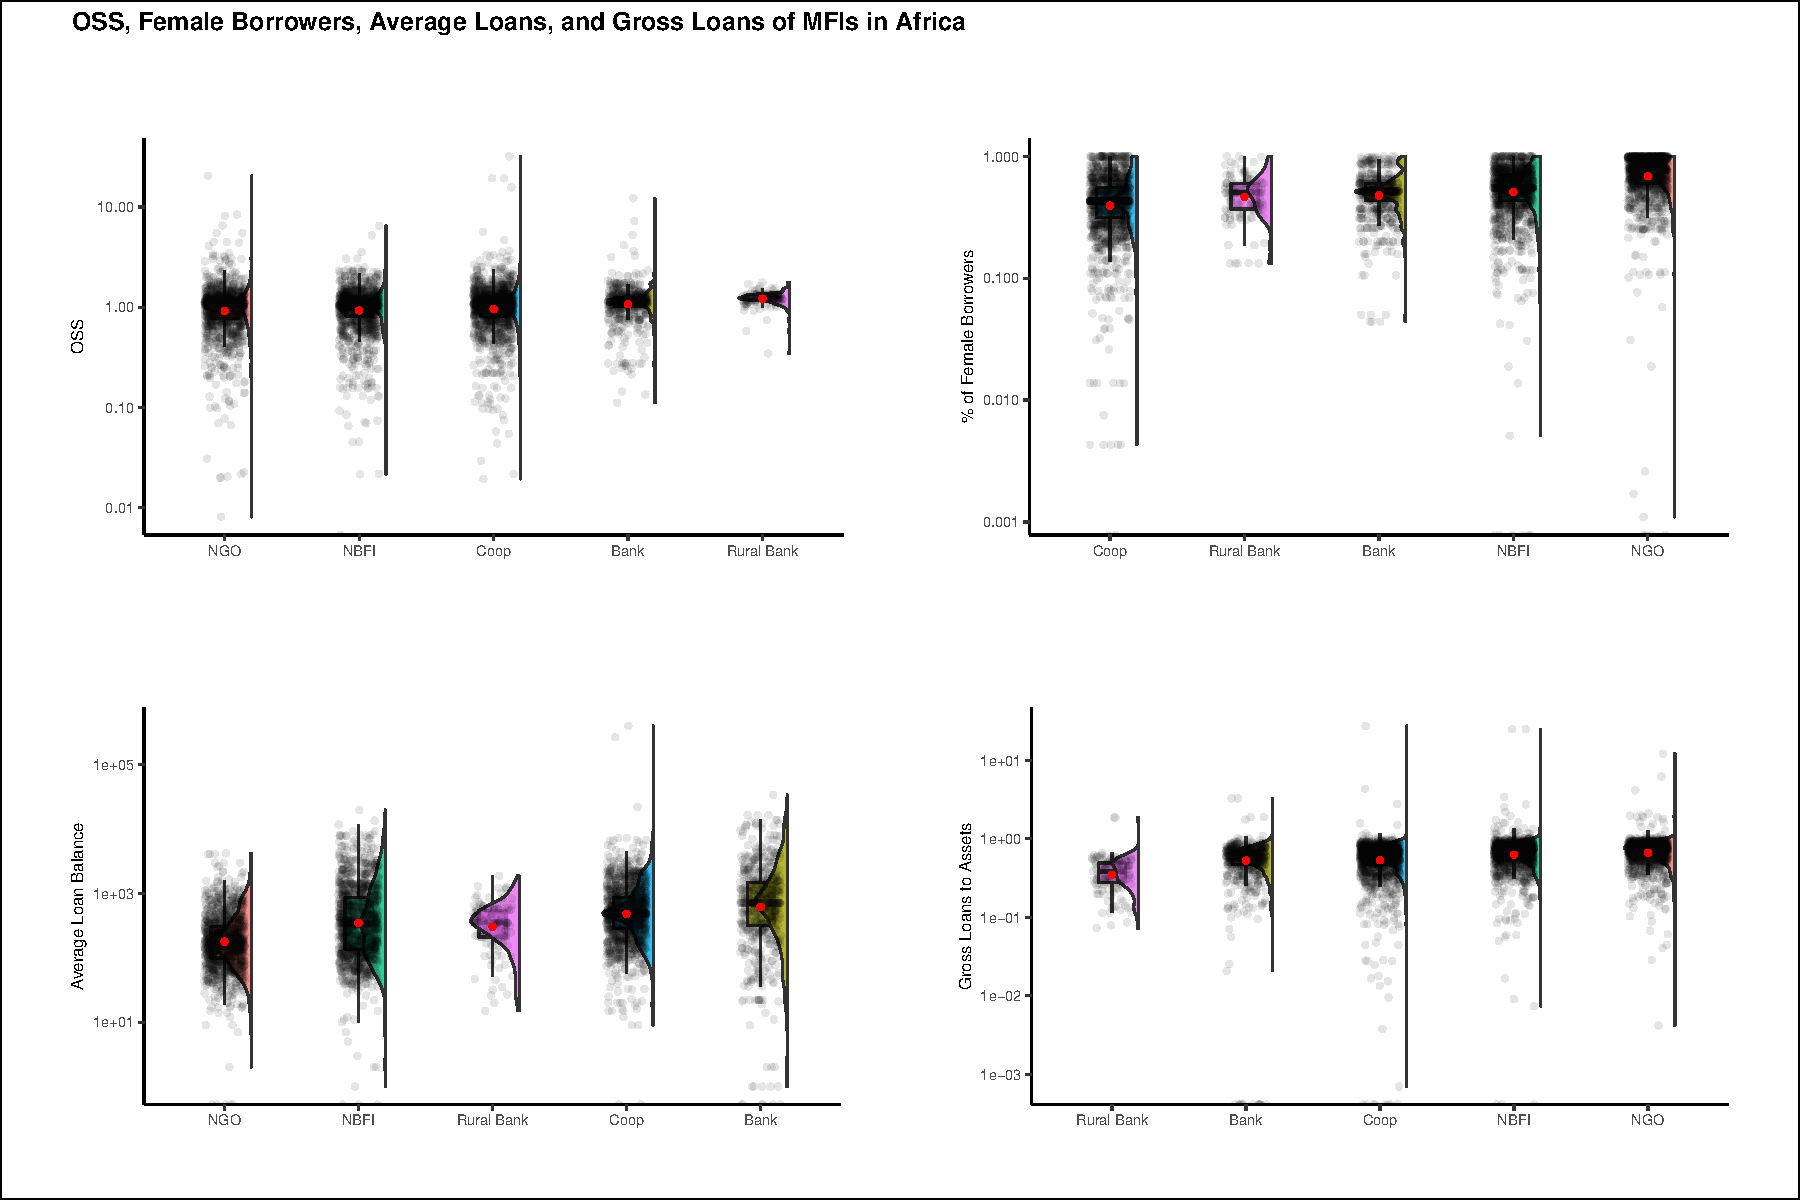
\includegraphics{finsoc_efficiency_files/figure-latex/unnamed-chunk-18-1.pdf}
\caption{Correlation Matrix for DEA Inputs and Outputs}
\end{figure}

\end{landscape}

\newpage

\hypertarget{independent-variables}{%
\subsection{Independent Variables}\label{independent-variables}}

Table 2 presents a summary of the independent variables applied in the
study.

\begin{longtabu} to \linewidth {>{\raggedright}X}
\caption{\label{tab:unnamed-chunk-19}Description of Independent Variables}\\
\toprule
Variable\_Description\\
\midrule
1. Current Legal Status: The legal forms of registration of an MFI are as follows; Commercial Bank, Non-Bank Financial Institution (NBFI), Non-Governmental Organization (NGO), Credit Union/ Cooperative, or Rural Bank. The legal status may dictate the profit orientation and sources of capital for the MFIs. The legal status of an MFI may impact the financing structure in several ways. First, legal status or form typically restricts NGOs from taking deposits, lowering the debt-equity ratio and deposits to assets, raising the capital asset ratio. Also, NGOs may not venture into capital markets for funds, given their not-for-profit orientation. The opposite is the case for MFIs of commercial banks legal form whose legal status allows for deposits.\\
\\
2.  Age: MIX classifies MFIs into three categories depending on the time that has elapsed since the MFI started operations- new (0-4 years), young (4-8 years) and mature (over eight years). The variable is hence a dummy. Older firms are likely better established, have a solid reputation and hence likely to attract more debt and deposits. The institutional life cycle view of Bayai and Ikhide (2016) captures the correspondence between age and debt.\\
\\
3. Legal Tradition (Legal): The indicator is a dummy variable with common law countries coded 0, civil law countries 1, and 2 otherwise as per the classification by Oto-Peralías and Romero-Ávila (2014). Typically, common law countries have relatively better financial infrastructure that allows firms to access financial markets easily. Hence, MFIs in common law countries may exhibit higher debt and equity ratios in their capital structures than those in common law and other legal traditions. (Schnyder, Gerhard, Mathias Siems, \& Ruth V. Aguilera, 2018)\\
\addlinespace
\\
4. Size (Log of Total Assets): We proxy the size of MFI with the natural logarithm of total assets, again using MIX data. Assets are supported by the sum of capital and liabilities or, equivalently, the total value of resources owned or controlled by the MFI resulting from past and current activities and from which the MFI derives future benefits. We expect firms with more assets to have a higher debt capacity and more debt-to-equity ratios, and lower capital to equity ratios. Large firms draw their strength from holding diversified investments and hence higher ability to absorb risk. Besides, they have easy access to debt markets(Kurshev \& Strebulaev, 2015). Furthermore, these firms are likely to attract more deposits, given the trust they inspire in depositors and their marketing reach (Kimmel et al., 2018). We hypothesise that donations vary positively with the size of MFI, as large, older firms have established a reputation with donors.\\
\\
5. Governance/ Institutional Quality (KKM): We create the country level KKM index using the first principal component of the WGI available in the World Bank databases. The index captures the institutional quality in corruption control, government effectiveness, political stability, the rule of law, and voice and accountability (Kaufmann, Kraay, \& Mastruzzi, 2011). Firms in countries with better governance can quickly raise debt finance due to ease of contract enforcement — the result, a high debt-equity ratio and a low capital asset ratio. Similarly, the level of deposits mobilisation may be higher in better-governed countries arising from consumer confidence in legislation relating to deposits protection (La Porta, Lopez-de-Silanes, \& Shleifer, 2013; Allen et al., 2014). Lastly, MFIs in countries with low KKM may have higher donations as donors opt to circumvent corrupt government channels. We use the terms institutional quality and governance interchangeably throughout the text\\
\\
\addlinespace
6. Private Credit to GDP: We capture the total amount of credit advanced to the private sector by financial intermediaries as a proxy for capital markets development concerning the banking sector following Ito and Kawai (2018). The data source is the Global Financial Development Database, GFDD, of the World Bank (See note 4). Private credit to GDP represents the financial resources provided to the private sector by domestic money banks as a share of GDP. Domestic money banks comprise commercial banks and other financial institutions that accept transferable deposits, such as demand deposits. The data is available in WDI. Financial sector development is central to the acquisition of both equity and debt financing. We hypothesise a high debt to equity ratio, and deposits to assets ratios in countries with more robust financial sectors as financial institutions tend to be highly leveraged.\\
\\
7. Stock market capitalisation to GDP: We capture the extent of stock market development using the ratio of stock market capitalisation to GDP to proxy how firms can raise equity capital. Although Africa's equity markets are thin, some relatively large stock markets like South Africa, Kenya, and Ghana exist. The data are from the GFDD.\\
\\
8. Asset Structure (Tangibility): Asset structure is is measured as the ratio of non-current assets to total assets of an MFI (Microfinance Information Exchange (MIX), 2019). The percentage indicates the extent of investment in physical infrastructure, a significant issue in constraining banking for the poor due to the perceived lack of scale economies to warrant the erection, for instance, of brick and mortar branches (Ledgerwood, 1998). MFIs with a more significant physical presence are likely to attract more deposits. Therefore, they also have a higher capacity to borrow and service debt. Further, tangible assets serve as collateral to protect lenders from the moral hazard problem (Jensen \& Meckling, 1976). Hence, there is a positive relationship between debt and asset tangibility (Titman \& Wessels, 1988; Kyereboah-Coleman, 2007a).\\
\addlinespace
\\
9. Profit Margin: The profit margin is the net operating income divided by financial revenue. The ratio represents the ability of MFIs to generate income from the core mandate of offering financial services like lending, savings, insurance, and so on. Profitability may enhance the capacity of an MFI to secure debt, thus leading to a higher debt to equity ratio and low capital to assets ratio. The opposite is the case when an MFI retains earnings and hence raises the level of equity.\\
\\
\bottomrule
\multicolumn{1}{l}{\rule{0pt}{1em}\textit{Source: }}\\
\multicolumn{1}{l}{\rule{0pt}{1em}Authors' construction from the literature}\\
\multicolumn{1}{l}{\rule{0pt}{1em}\textit{Notes}}\\
\multicolumn{1}{l}{\rule{0pt}{1em}\textsuperscript{1} MIX Database on www.themix.org and https://datacatalog.worldbank.org/dataset/mix-market}\\
\multicolumn{1}{l}{\rule{0pt}{1em}\textsuperscript{2} WDI on https://databank.worldbank.org/source/world-development-indicators.}\\
\multicolumn{1}{l}{\rule{0pt}{1em}\textsuperscript{3} WGI/ KKM on https://databank.worldbank.org/source/worldwide-governance-indicators.}\\
\multicolumn{1}{l}{\rule{0pt}{1em}\textsuperscript{4} GFDD on https://www.worldbank.org/en/publication/gfdr/data/global-financial-development-database}\\
\end{longtabu}

\hypertarget{results}{%
\section{Results}\label{results}}

\hypertarget{exploratory-data-analysis}{%
\subsection{Exploratory Data Analysis}\label{exploratory-data-analysis}}

We examine the indicators of financial and social performance by MFIs in
Africa. Here, we focus on taking individual performance measures, the
proportion of female borrowers, average loan balance per borrower, gross
loans to assets, and operational self-sufficiency. While the examination
of indicator variables does not explicitly measure efficiency (we do
this in a later section using DEA), they illustrate the extent to which
MFIs fare in their mission:

\begin{enumerate}
\def\labelenumi{\arabic{enumi}.}
\tightlist
\item
  Table 2 (above) presents the descriptive statistics. We visualise the
  data and describe the scope of financial and social performance,
  followed by a discussion of the DEA efficiency scores.
\item
  We discuss the levels of efficiency by MFIs types based on the DEA
  scores.
\item
  We layout and describe the results of the regression model.
\end{enumerate}

\hypertarget{dea-efficiency-scores}{%
\subsubsection{DEA Efficiency Scores}\label{dea-efficiency-scores}}

Table 3 shows summary statistics of the efficiency scores for MFIs in
Africa. Given that the model is output-oriented, the interpretation is
as follows: given a set of inputs, to what extent are MFIs able to
maximise output? Given that the study targets the extent of financial
inclusion and financial sustainability of MFIs, the maximisation of
outputs is more relevant for this study.

\hypertarget{financial-efficiency-1}{%
\paragraph{Financial Efficiency}\label{financial-efficiency-1}}

Table () shows a summary of the efficiency scores. The mean and median
financial efficiency scores are 0.16 and 0.11, respectively.\footnote{The
  DEA scores range between zero and one, with zero indicating the worst
  performance and one the best.} Taken together with Figure 2, the
results show that the financial efficiency scores skew heavily to the
right. Critically, MFIs are hardly financially sustainable regardless of
their legal form, despite the paradigm shift towards commercialization.
This observation begs the two questions; do commercially oriented legal
forms of MFIs perform better than NGOs? Further, do newer MFIs that took
root when donors emphasize the financial sustainability of MFIs do
better financially than older MFIs?

Figure 2, panel C shows that only cooperatives and rural banks have
higher median financial efficiency scores than NGOs. These results do
not support the supposition that commercialization raises financial
sustainability, given that commercial banks and NBFIs fare worse
financially. The poor financial performance by banks and NBFIs can only
further worsen their outreach to the financially excluded. The poor
financial performance is contrary to the ``mission expansion''
hypothesis where commercial MFIs generate profits that they then use to
reach more financially excluded clients. Further, in Figure 2, panel D
shows that newer MFIs have higher financial sustainability scores
relative to older MFIs. These results could mean that newer MFIs focus
more on financial sustainability at the expense of social goals or are
better at balancing financial sustainability with social goals.

Figure (), panel () shows the trends in median financial efficiency
scores of MFIs for 1999-2020. Cooperatives consistently do better
financially than other legal forms. Surprisingly, NGOs and rural banks
follow, while NBFIs and commercial banks have the lowest median
financial efficiency scores, with commercial banks showing wide
variability. The results indicate that commercialization does not
necessarily raise financial sustainability, especially in the absence of
grants and state subsidies. What is concerning is the observation that
financial efficiency is on a downward spiral, meaning that MFIs may not
achieve the goal of financial sustainability of MFIs. The worsening
trend in financial performance by MFIs may point to the harm that
neo-liberalism, commercialization, or other unidentified macro-economic
factors have on MFIs.

\begin{table}

\caption{\label{tab:unnamed-chunk-20}Summary Statistics for Efficiency Scores}
\centering
\fontsize{10}{12}\selectfont
\begin{tabular}[t]{lrrrrrrr}
\toprule
Variable & Mean & SD & Min & Q1 & Median & Q3 & Max\\
\midrule
financial Efficiency & 0.1572 & 0.1892 & 0.0292 & 0.0944 & 0.1079 & 0.1272 & 1\\
Social Efficiency & 0.7862 & 0.1186 & 0.5000 & 0.7126 & 0.7767 & 0.8750 & 1\\
Financial and Social Efficiency & 0.7947 & 0.1228 & 0.5000 & 0.7146 & 0.7767 & 0.8938 & 1\\
\bottomrule
\end{tabular}
\end{table}

\begin{landscape}

\newpage

\begin{figure}
\centering
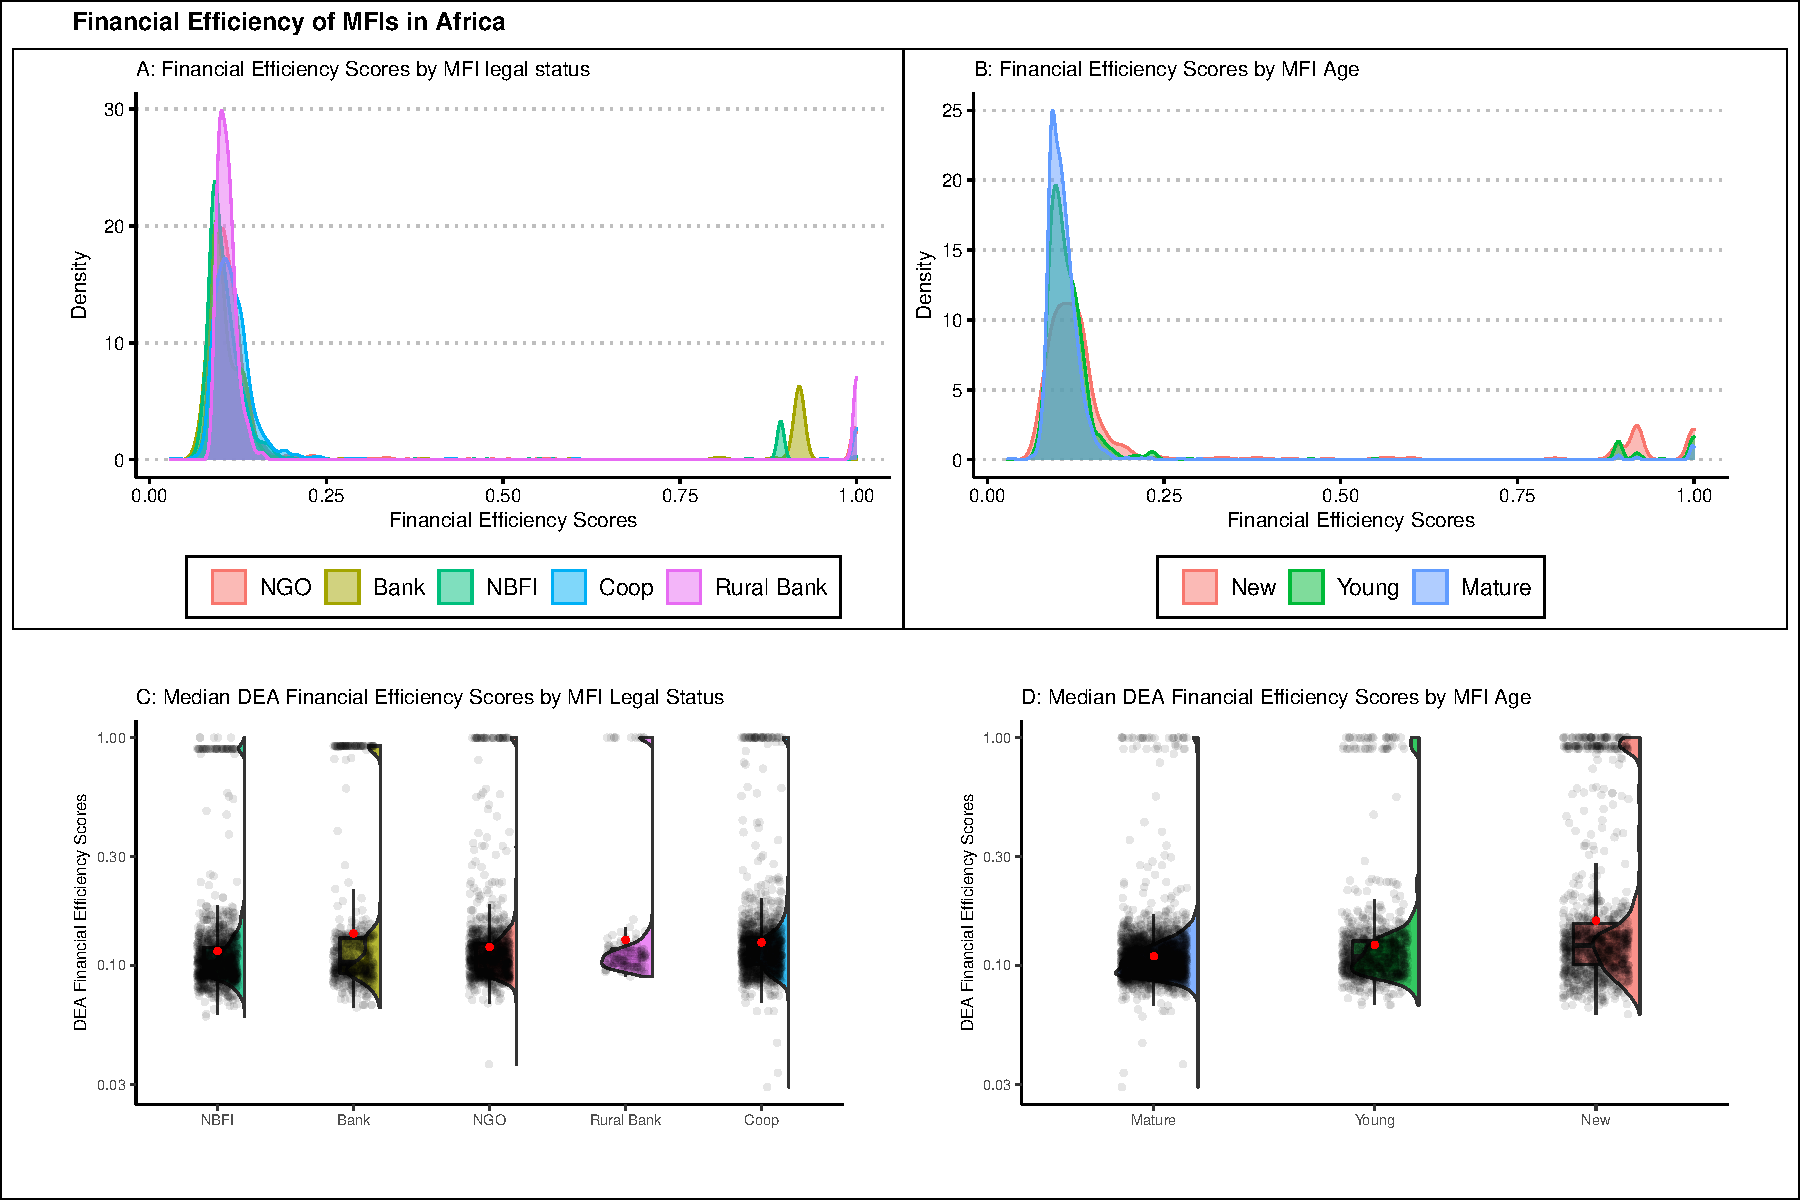
\includegraphics{finsoc_efficiency_files/figure-latex/unnamed-chunk-21-1.pdf}
\caption{Financial Efficiency Scores for MFIs in Africa}
\end{figure}

\end{landscape}

\newpage

\hypertarget{social-efficiency-1}{%
\paragraph{Social Efficiency}\label{social-efficiency-1}}

Overall, the social efficiency of MFIs in Africa is high, with a mean
and median of 0.79 and 0.78, respectively. However, as Figure () and ()
show, NGOs have consistently the highest levels of social efficiency,
followed by NBFIs and other forms of MFIs. Rural banks and credit
unions, respectively, are the least socially efficient. Considering the
financial efficiency scores, it appears that commercialization causes
mission drift. Also, both NGOs and NBFIs show a notable decline in
social performance over time, which could also be an indictment of the
shift towards financial sustainability.

An important observation is that younger MFIs have a higher level of
social performance than mature MFIs. Earlier, we saw that younger MFIs
also have better financial performance than older MFIs. The implication
is that younger MFIs are better at balancing financial and social goals
than mature MFIs. The explanation could be that younger MFIs have
developed their business model in the face of declining donor support or
the complete absence of donor funding and state subsidies. Older MFIs
required to shift from the donor and state subsidy reliant model to the
commercial model do not perform well. Given that mature MFIs are larger
and reach more financially excluded clients, the issue is how to support
mature MFIs to transition to the financial sustainability model without
reducing their outreach.

\begin{landscape}

\begin{figure}
\centering
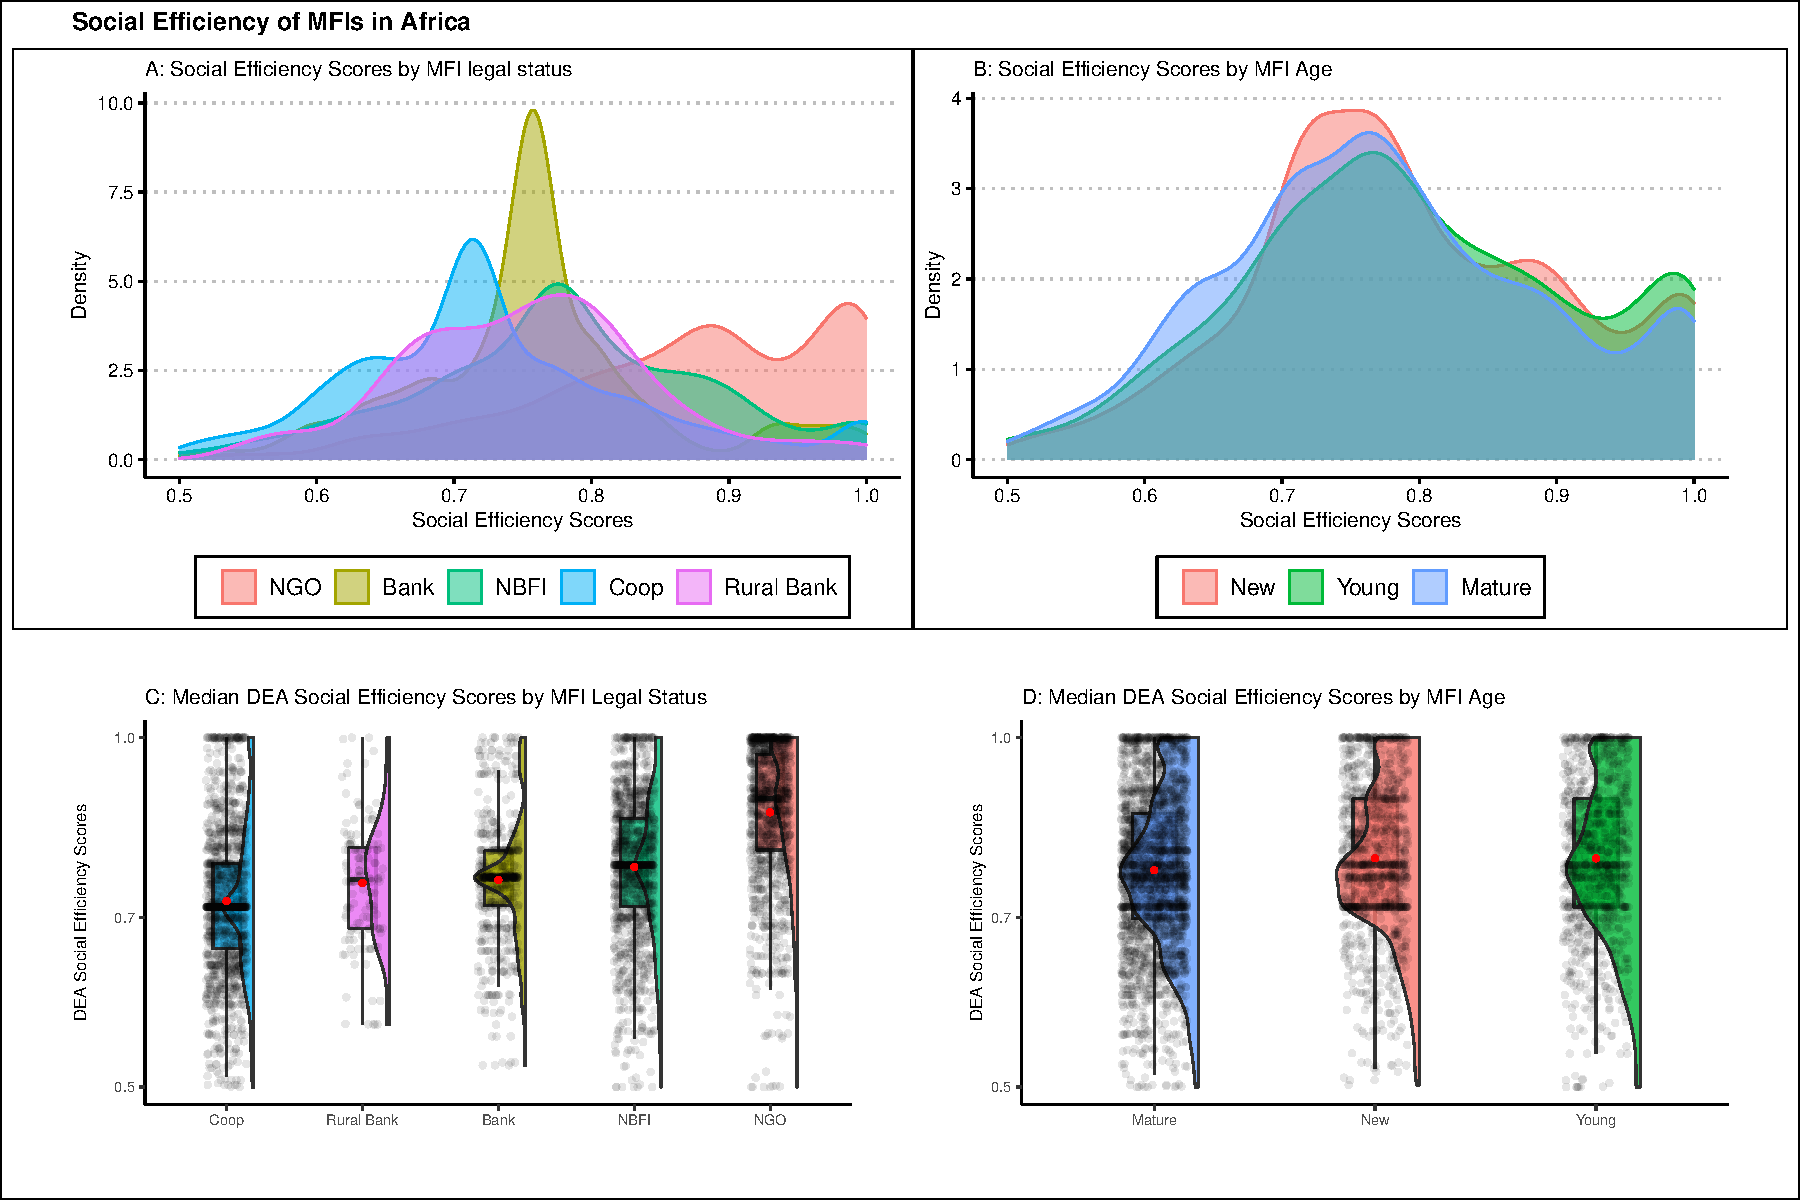
\includegraphics{finsoc_efficiency_files/figure-latex/unnamed-chunk-22-1.pdf}
\caption{Social Efficiency Scores for MFIs in Africa}
\end{figure}

\end{landscape}

\hypertarget{financial-and-social-efficiency-scores}{%
\paragraph{Financial and Social Efficiency
Scores}\label{financial-and-social-efficiency-scores}}

In Figure (), we combine the social and financial metrics. The DEA model
now captures the efficiency with which MFIs in Africa convert the inputs
(liabilities and equity) into outputs (average loan balance per
borrower, percentage of women borrowers, and operational
self-sufficiency, OSS). Table () shows the summary statistics of the DEA
analysis. The socio-financial efficiency scores are high, with a median
of 0.7947 and a mean of 0.7767. Again, the median financial efficiency
metric is highest for NGOs, which is an oddity for we expect commercial
firms to dominate (see panels A and C). These results mean that NGOs are
better at balancing microfinance's financial and social goals than
commercial MFIs. NBFIs, banks, rural banks, and cooperatives follow in
that order. These results seem like an indictment of the conversion of
MFIs to the commercial model.

In Figure (), panels B and D, we plot the median financial and social
performance of MFIs faceted by age. As in the social and financial
efficiency analysis, younger MFIs fare better in socio-financial
efficiency scores than do older MFIs. Again, these results imply that
younger MFIs are better at balancing the social and financial aspects of
microfinance, as discussed before. Figure (), panel D shows the trends
in the socio-financial efficiency of MFIs. While the scores appear
stable across time, NGOs score consistently higher. Overall, these
results mean that embracing neo-liberalism may be harming social
performance without helping improve financial performance.

\begin{landscape}

\newpage

\begin{figure}
\centering
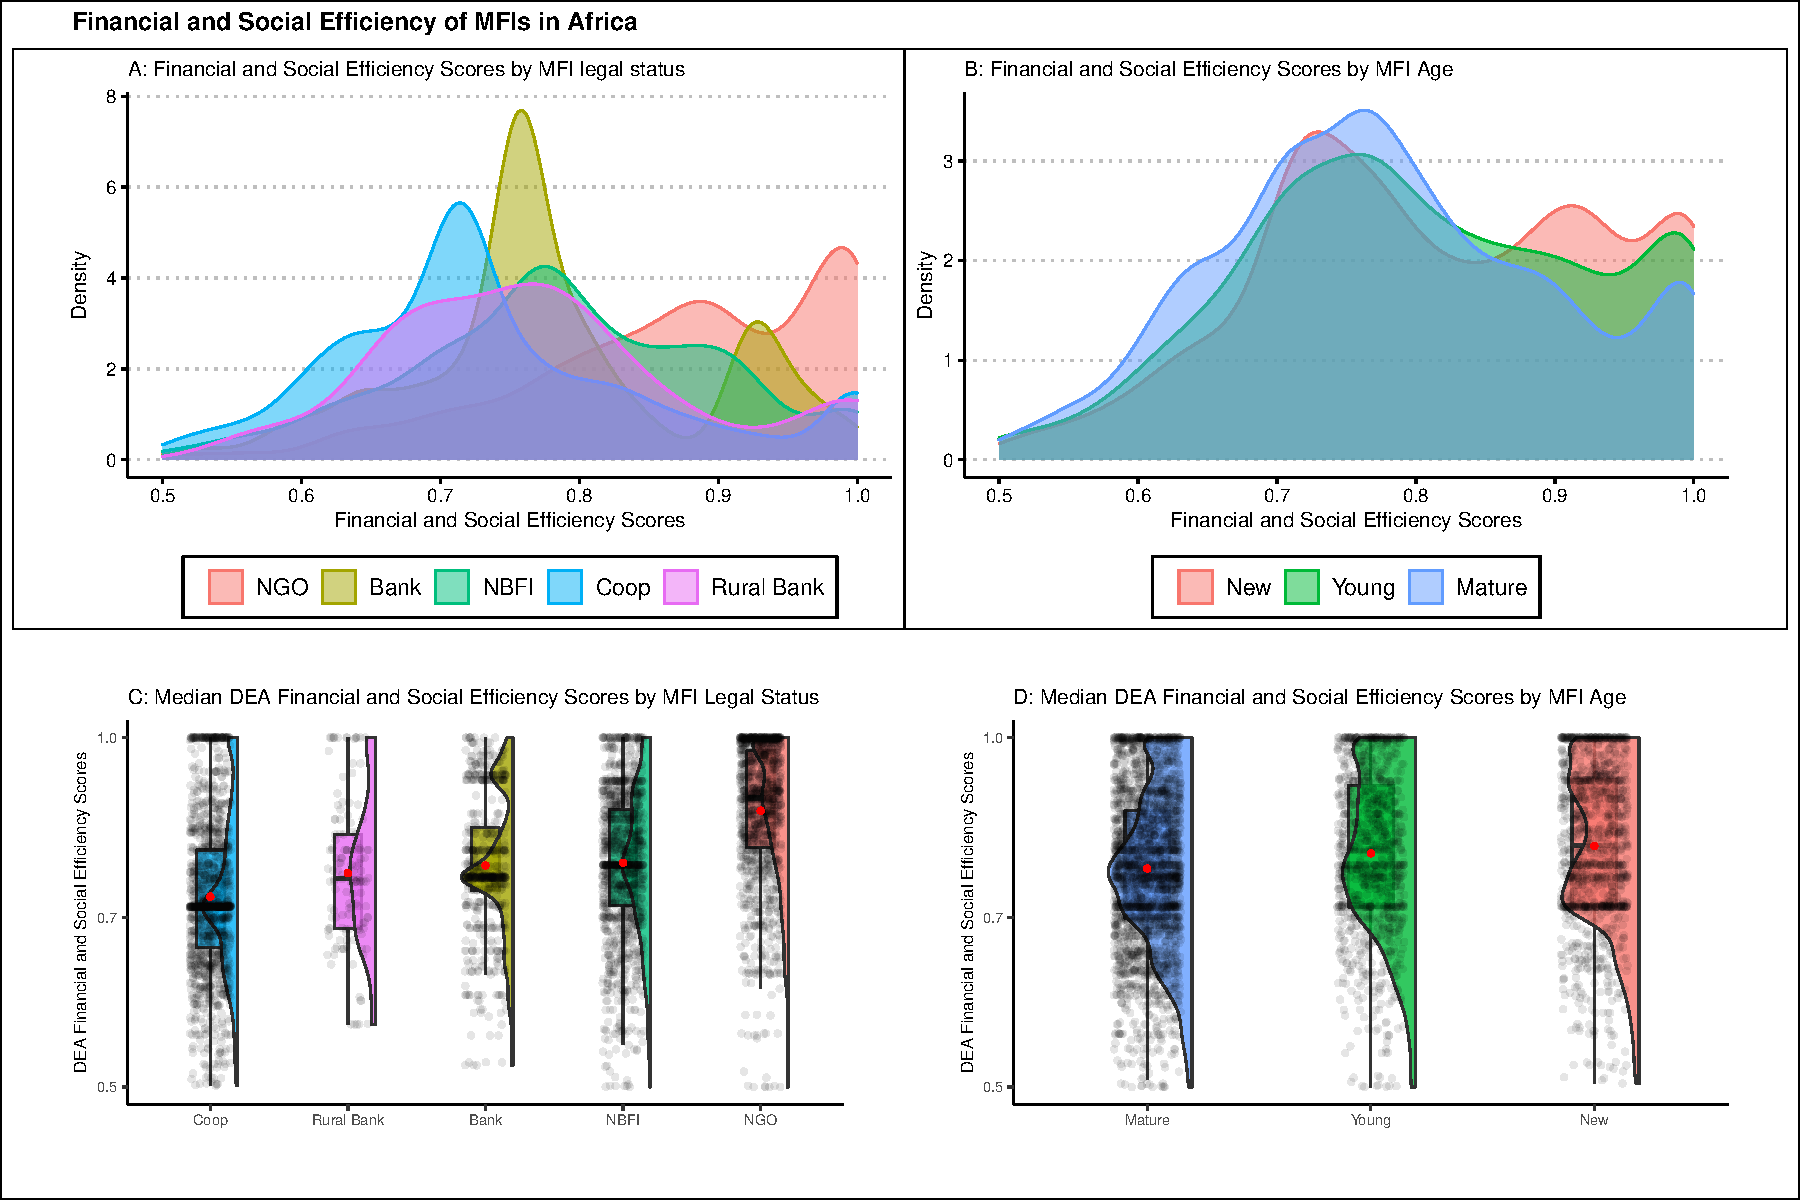
\includegraphics{finsoc_efficiency_files/figure-latex/unnamed-chunk-23-1.pdf}
\caption{Financial and Social Efficiency Scores for MFIs in Africa}
\end{figure}

\end{landscape}

\newpage

\begin{landscape}

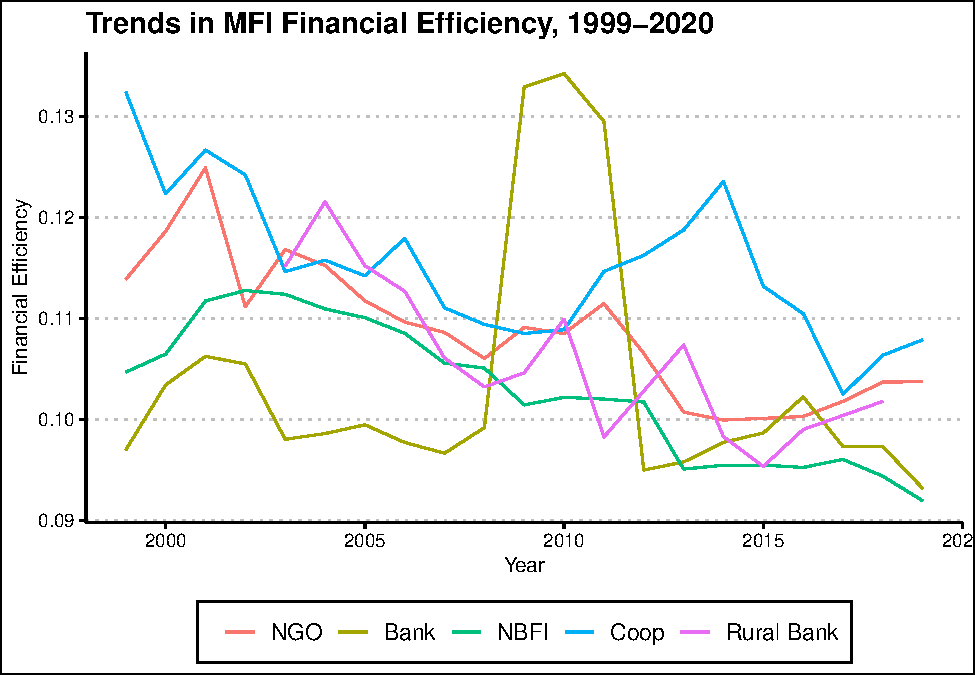
\includegraphics{finsoc_efficiency_files/figure-latex/unnamed-chunk-24-1.pdf}

\end{landscape}

\hypertarget{the-independent-variables}{%
\subsubsection{The Independent
Variables}\label{the-independent-variables}}

Table () shows summary statistics for the independent variables. Profit
margin has the highest variability due to extreme minimum observation.
To proxy the size of an MFI, we take the logarithm of assets. We use all
the other independent variables without transformation.

\begin{table}

\caption{\label{tab:unnamed-chunk-25}Summary Statistics: Independent Variables for Regression Model}
\centering
\fontsize{10}{12}\selectfont
\begin{tabular}[t]{lrrrrrrr}
\toprule
Variable & Mean & SD & Min & Q1 & Median & Q3 & Max\\
\midrule
Asset Structure & 0.0759 & 0.0694 & 0.000e+00 & 0.0351 & 0.0599 & 0.092 & 0.8598\\
KKM & 0.0026 & 2.0064 & -5.233e+00 & -1.3041 & -0.1137 & 1.628 & 7.3690\\
Private Credit & 2.7194 & 0.6852 & 2.981e-01 & 2.3864 & 2.7584 & 3.052 & 6.8806\\
Stock Market & 1.1410 & 1.4732 & 0.000e+00 & 0.0000 & 0.0000 & 2.428 & 5.7972\\
Profit Margin & -7.7393 & 513.2995 & -3.550e+04 & -0.1814 & 0.0484 & 0.189 & 6.2019\\
\addlinespace
Assets & 14.9461 & 2.2619 & 6.931e-01 & 13.5399 & 14.8577 & 16.416 & 22.9786\\
\bottomrule
\multicolumn{8}{l}{\rule{0pt}{1em}Source: Authors construction from the data}\\
\multicolumn{8}{l}{\rule{0pt}{1em}\textit{Note: }}\\
\multicolumn{8}{l}{\rule{0pt}{1em}\textsuperscript{1} Private credit refers to credit advanced by deposit taking banks as a percentage of GDP}\\
\multicolumn{8}{l}{\rule{0pt}{1em}\textsuperscript{2} Stock market is the stock market capitalisation as a percentage of GDP}\\
\end{tabular}
\end{table}

In the next section, we detail the regression output from the drivers of
the efficiency of MFIs in Africa.

\hypertarget{regression-analysis}{%
\section{Regression Analysis}\label{regression-analysis}}

In this section, we regress each of the DEA efficiency scores against
the dependent variables. We bootstrap the DEA efficiency scores before
applying them to the regression model (Simar and Wilson 2000; Tziogkidis
2012; Fethi and Pasiouras 2010). The purpose of using the bootstrapping
approach is two-fold: first, to obtain the bias-corrected estimates and
the confidence intervals of DEA-efficiency scores and second, to
overcome the correlation problem of DEA-efficiency scores and to provide
consistent inferences in explaining the determinants of financial and
social efficiency (Assaf and Matawie 2010). The bootstrapped DEA scores
serve as the dependent variables in the regression analysis. This
section provides results from the regression models on the drivers of
the socio-financial efficiency of MFIs in Africa.

\hypertarget{financial-efficiency-of-mfis}{%
\subsection{Financial Efficiency of
MFIs}\label{financial-efficiency-of-mfis}}

Table () shows the results of the regression analysis with financial
efficiency as the dependent variable. The significant drivers of
financial efficiency are asset structure, MFI size proxied by the
logarithm of total assets, and stock market capitalisation to GDP.
Current legal status has a weak relationship with financial efficiency.
The regression analysis shows that commercial banks and rural banks have
significantly better financial efficiency, which goes against the
visualisation in table (). The extreme values in the financial
performance of banks and rural banks could explain this contradiction.
But overall, NGOs do better financially than all the legal forms of MFIs
except cooperatives.

These results go against the stated objectives of MFI commercialisation.
The commercial model of microfinance aims at increasing the financial
sustainability of MFIs, which would allow for their sustainability
without reliance on donations and subsidies. Again, financial
sustainability by MFIs would lead to mission expansion by using profits
to teach the financially excluded. However, the data shows that this is
not the case. Overall, the financial performance of MFIs is poor.
However, the commercial MFIs do not outperform NGOs in financial
performance in the sample dataset. It then seems like commercialisation
does not necessarily translate into financial sustainability. And given
the relatively good financial performance by NGOs that do not explicitly
prioritise profitability, it appears that the win-win school has the
upper hand. MFIs can balance financial and social goals while retaining
the NGO model that focuses on social goals.

The asset structure of MFIs has an inverse relationship with financial
efficiency. As noted earlier, asset structure or asset tangibility is
the ratio of non-current assets to total assets of an MFI. The results
then imply that investment in physical infrastructure harms financial
sustainability (Iman, 2018, Demirguc-Kunt et al., 2018). The results are
consistent with the theory because serving the financially excluded is
expensive and may not yield economies of scale to offset the investment
in physical infrastructure by MFIs.

The advent of Fintech allows MFIs to reach out to the financially
excluded without high expenditures in brick and mortar branches and
other physical assets. However, given that most financially excluded
people also suffer from financial illiteracy, MFIs still must deploy
field workers or mobile banking units in targeted areas. (Allen et al.,
2014). Hence, there is an opportunity for research into how Fintech
affects the investment in physical infrastructure, profitability and
outreach of MFIs in Africa.

The size of an MFI is also negatively related to the financial
efficiency of MFIs in Africa. Large, older MFIs have lower financial
efficiency scores relative to smaller, younger, which could arise due to
dis-economies of scale. Also, larger, older MFIs may not emphasise
financial sustainability, given they receive relatively more donations.
If donors emphasise outreach to financial sustainability, this could
explain the lower levels of financial performance by older MFIs. The
ratio of stock market capitalisation to GDP has a weak positive
relationship with financial efficiency, implying that MFIs operating in
countries with better functioning capital markets exhibit better
financial performance. The ratio of private credit to GDP is
insignificant. The remaining variables, age and institutional quality,
have no significant relationship with financial efficiency. However, as
we saw earlier in table (), younger MFIs have marginally higher
financial performance, which is not significant in the regression.

\newpage

\begin{landscape}

\begin{table}[!htbp] \centering 
  \caption{Regression Output for Financial Efficiency (Standard Errors in Brackets)} 
  \label{} 
\footnotesize 
\begin{tabular}{@{\extracolsep{5pt}}lD{.}{.}{-3} D{.}{.}{-3} D{.}{.}{-3} D{.}{.}{-3} D{.}{.}{-3} D{.}{.}{-3} } 
\\[-1.8ex]\hline 
\hline \\[-1.8ex] 
 & \multicolumn{6}{c}{\textit{Dependent variable:}} \\ 
\cline{2-7} 
\\[-1.8ex] & \multicolumn{6}{c}{depvar} \\ 
\\[-1.8ex] & \multicolumn{1}{c}{(1)} & \multicolumn{1}{c}{(2)} & \multicolumn{1}{c}{(3)} & \multicolumn{1}{c}{(4)} & \multicolumn{1}{c}{(5)} & \multicolumn{1}{c}{(6)}\\ 
\hline \\[-1.8ex] 
 currentlegalstatusBank &  &  &  & 0.127^{***} & 0.012 & 0.028^{**} \\ 
  &  &  &  & (0.025) & (0.020) & (0.013) \\ 
  & & & & & & \\ 
 currentlegalstatusNBFI &  &  &  & 0.019 & -0.006 & 0.005 \\ 
  &  &  &  & (0.019) & (0.015) & (0.009) \\ 
  & & & & & & \\ 
 currentlegalstatusCoop & -0.002 & -0.001 & -0.0004 & -0.003 & -0.005 & 0.008 \\ 
  & (0.019) & (0.018) & (0.022) & (0.015) & (0.014) & (0.009) \\ 
  & & & & & & \\ 
 currentlegalstatusRural Bank &  &  &  & 0.053^{*} & -0.038 & -0.004 \\ 
  &  &  &  & (0.031) & (0.028) & (0.028) \\ 
  & & & & & & \\ 
 ageYoung & 0.002 & 0.001 & 0.002 & 0.001 & 0.001 & 0.002 \\ 
  & (0.002) & (0.002) & (0.002) & (0.003) & (0.003) & (0.002) \\ 
  & & & & & & \\ 
 ageMature & 0.005^{*} & 0.004 & 0.005 & 0.002 & 0.003 & 0.004 \\ 
  & (0.003) & (0.003) & (0.003) & (0.003) & (0.003) & (0.003) \\ 
  & & & & & & \\ 
 kkm & -0.002 & -0.002^{*} & -0.002 & -0.0001 & -0.001 & 0.0004 \\ 
  & (0.001) & (0.001) & (0.001) & (0.001) & (0.001) & (0.001) \\ 
  & & & & & & \\ 
 asset\_structure & -0.070^{***} & -0.060^{***} & -0.066^{***} & -0.087^{***} & -0.069^{***} & -0.067^{***} \\ 
  & (0.015) & (0.016) & (0.016) & (0.018) & (0.017) & (0.016) \\ 
  & & & & & & \\ 
 pcrdbgdp & -0.001 & 0.002 & 0.002 & -0.002 & -0.003 & -0.004 \\ 
  & (0.003) & (0.003) & (0.003) & (0.004) & (0.004) & (0.003) \\ 
  & & & & & & \\ 
 stmktcap & 0.004^{*} & 0.004 & 0.007^{***} & 0.005^{**} & 0.003 & 0.005^{***} \\ 
  & (0.002) & (0.002) & (0.002) & (0.003) & (0.002) & (0.002) \\ 
  & & & & & & \\ 
 log(assets) & -0.159^{***} & -0.138^{***} & -0.128^{***} & -0.183^{***} & -0.152^{***} & -0.127^{***} \\ 
  & (0.012) & (0.012) & (0.017) & (0.013) & (0.013) & (0.016) \\ 
  & & & & & & \\ 
\hline \\[-1.8ex] 
Model & Within & Within & Within & Random & Random & Random \\ 
Data & Full & >=3 Years & >=5 Years & Full & >=3 Years & >=5 Years \\ 
Observations & \multicolumn{1}{c}{4,782} & \multicolumn{1}{c}{3,840} & \multicolumn{1}{c}{3,165} & \multicolumn{1}{c}{4,782} & \multicolumn{1}{c}{3,840} & \multicolumn{1}{c}{3,165} \\ 
R$^{2}$ & \multicolumn{1}{c}{0.078} & \multicolumn{1}{c}{0.073} & \multicolumn{1}{c}{0.098} & \multicolumn{1}{c}{0.151} & \multicolumn{1}{c}{0.095} & \multicolumn{1}{c}{0.101} \\ 
Adjusted R$^{2}$ & \multicolumn{1}{c}{-0.142} & \multicolumn{1}{c}{-0.057} & \multicolumn{1}{c}{-0.003} & \multicolumn{1}{c}{0.146} & \multicolumn{1}{c}{0.088} & \multicolumn{1}{c}{0.093} \\ 
F Statistic & \multicolumn{1}{c}{11.630$^{***}$ (df = 28; 3862)} & \multicolumn{1}{c}{9.522$^{***}$ (df = 28; 3366)} & \multicolumn{1}{c}{11.080$^{***}$ (df = 28; 2845)} & \multicolumn{1}{c}{380.100$^{***}$} & \multicolumn{1}{c}{281.000$^{***}$} & \multicolumn{1}{c}{293.000$^{***}$} \\ 
\hline 
\hline \\[-1.8ex] 
\textit{Note:}  & \multicolumn{6}{r}{$^{*}$p$<$0.1; $^{**}$p$<$0.05; $^{***}$p$<$0.01} \\ 
\end{tabular} 
\end{table}

\end{landscape}

\newpage

\hypertarget{drivers-of-social-efficiency-of-mfis}{%
\subsection{Drivers of Social Efficiency of
MFIs}\label{drivers-of-social-efficiency-of-mfis}}

Unlike financial performance, the legal form of an MFI is the dominant
driver of social performance. Consistent with figure (), NGOs have
significantly higher social performance levels than all the other legal
forms of MFIs. The concern by the welfare school of microfinance is that
the levels of outreach by NGOs to the financially excluded could be
affected by focusing on financial sustainability. However, as the
previous section shows, NGOs do not fare badly in financial efficiency
than other legal forms of MFIs. It means, therefore, that NGOs could aim
at a degree of financial efficiency while still maintaining their social
goals. As Mersland, Nyarko, and Szafarz (2019) note, the mission
statements of MFIs have a significant relationship with the performance
of these MFIs. Given that NGOs have the stated mission of reaching the
unbanked, they are better positioned to achieve these social goals. If
NGOs are to give financial goals as much weight as social goals, there
is likely to be a trade-off, more so where fund providers put pressure
on management to make financial returns.

The results are consistent with the data visualisations. Credit unions
have the objective of serving subscribed members within a designated
geographic location or a common professional background. It is not their
mission to explicitly target social performance (Mathuva, Mboya, and
McFie 2017). The contestation here is between NGOs and the other
commercial entities, excluding credit unions. The results illustrate
that MFIs that exclusively target social performance tend to achieve
more socially. Hence the place of the social mission of an MFI is
central to achieving social objectives, a view that is in line with
findings by Berbegal-Mirabent, Mas-Machuca, and Guix (2019).

Both stock markets capitalisation to GDP and private credit to GDP have
a negative and significant relationship with social performance. These
two metrics capture the levels of capital market development. People in
countries with higher levels of financial development have lower
incidences of financial exclusion, on average, relative to people in
countries with lower levels of financial inclusion. This observation is
despite the concurrence in the literature that the ability to access
financial services does not necessarily translate into the usage of
financial services. However, access to financial services is a necessary
precondition for people to use financial services. Financial development
means better financial infrastructure that allows people who could
otherwise not use financial services because of lack of access to these
services.

Institutional quality (KKM) has a mixed but insignificant relationship
with the social performance of MFIs. As expected, asset structure has a
positive, albeit insignificant relationship with social performance,
given that MFIs that have a greater presence in financially under-served
communities would tend to serve more financially excluded clients.
Likewise, the size of an MFI shows a positive but insignificant
relationship with social outreach.

Again, consistent with the data visualisation, younger MFIs have better
levels of social performance than older MFIs, although the coefficients
are not significant in the regression. The result seems odd because
younger MFIs started when the sustainability school was gaining ground,
meaning low donations and subsidies. But given that younger MFIs are
smaller, they may serve geographically limited areas to serve more
financially excluded clients. The broader coverage by older MFIs makes
it hard for them to focus on social goals, given the financial
implications of sustaining their presence in these settings.

\hypertarget{socio-financial-efficiency-of-mfis}{%
\subsection{Socio-Financial Efficiency of
MFIs}\label{socio-financial-efficiency-of-mfis}}

In this regression model, we examine joint social and financial
efficiency (socio-financial efficiency). Specifically, we seek to
uncover how well MFIs convert their inputs into financial (operational
self-sufficiency) and social goals (percentage of female borrowers and
average loan balance per borrower). The results show that, like social
efficiency, the statistically significant drivers of socio-financial
efficiency are legal status and the ratio of stock market capitalisation
to GDP. Specifically, the regression analysis shows that NGOs have
higher socio-financial efficiency scores than the other legal forms of
MFIs, confirming the results of exploratory data analysis. These results
suggest that transformed MFIs do not achieve the attained benefits of
commercialisation- increased financial sustainability, which allows for
greater outreach to the financially excluded (mission expansion).
Instead, it is NGOs that are capable of balancing financial and social
goals. Like in social goals, socio-financial efficiency has a negative
relationship with stock market capitalisation to GDP, highlighting the
importance of financial sector development in enabling financial
inclusion.

\begin{landscape}

\newpage

\begin{table}[!htbp] \centering 
  \caption{Regression Output for Social Efficiency (Standard Errors in Brackets)} 
  \label{} 
\footnotesize 
\begin{tabular}{@{\extracolsep{5pt}}lD{.}{.}{-3} D{.}{.}{-3} D{.}{.}{-3} D{.}{.}{-3} D{.}{.}{-3} D{.}{.}{-3} } 
\\[-1.8ex]\hline 
\hline \\[-1.8ex] 
 & \multicolumn{6}{c}{\textit{Dependent variable:}} \\ 
\cline{2-7} 
\\[-1.8ex] & \multicolumn{6}{c}{depvar} \\ 
\\[-1.8ex] & \multicolumn{1}{c}{(1)} & \multicolumn{1}{c}{(2)} & \multicolumn{1}{c}{(3)} & \multicolumn{1}{c}{(4)} & \multicolumn{1}{c}{(5)} & \multicolumn{1}{c}{(6)}\\ 
\hline \\[-1.8ex] 
 currentlegalstatusBank &  &  &  & -0.106^{***} & -0.096^{***} & -0.095^{***} \\ 
  &  &  &  & (0.014) & (0.020) & (0.022) \\ 
  & & & & & & \\ 
 currentlegalstatusNBFI &  &  &  & -0.084^{***} & -0.080^{***} & -0.077^{***} \\ 
  &  &  &  & (0.011) & (0.014) & (0.015) \\ 
  & & & & & & \\ 
 currentlegalstatusCoop & 0.047 & 0.048 & 0.048 & -0.137^{***} & -0.122^{***} & -0.124^{***} \\ 
  & (0.054) & (0.057) & (0.063) & (0.010) & (0.014) & (0.017) \\ 
  & & & & & & \\ 
 currentlegalstatusRural Bank &  &  &  & -0.103^{***} & -0.124^{***} & -0.130^{**} \\ 
  &  &  &  & (0.022) & (0.033) & (0.052) \\ 
  & & & & & & \\ 
 ageYoung & -0.001 & -0.003 & -0.001 & -0.002 & -0.003 & -0.001 \\ 
  & (0.005) & (0.005) & (0.006) & (0.004) & (0.005) & (0.006) \\ 
  & & & & & & \\ 
 ageMature & -0.004 & -0.005 & -0.002 & -0.006 & -0.008 & -0.003 \\ 
  & (0.007) & (0.008) & (0.009) & (0.006) & (0.007) & (0.009) \\ 
  & & & & & & \\ 
 kkm & 0.0004 & 0.0003 & -0.0002 & -0.001 & -0.003 & -0.003 \\ 
  & (0.003) & (0.003) & (0.004) & (0.002) & (0.002) & (0.003) \\ 
  & & & & & & \\ 
 asset\_structure & 0.024 & 0.029 & 0.036 & 0.010 & 0.022 & 0.029 \\ 
  & (0.029) & (0.034) & (0.042) & (0.027) & (0.032) & (0.040) \\ 
  & & & & & & \\ 
 pcrdbgdp & -0.011 & -0.013 & -0.013 & -0.009^{*} & -0.011^{*} & -0.010 \\ 
  & (0.007) & (0.008) & (0.009) & (0.005) & (0.007) & (0.007) \\ 
  & & & & & & \\ 
 stmktcap & -0.013^{***} & -0.014^{***} & -0.012^{**} & -0.002 & -0.002 & -0.004 \\ 
  & (0.004) & (0.004) & (0.005) & (0.003) & (0.003) & (0.004) \\ 
  & & & & & & \\ 
 log(assets) & 0.026 & 0.035 & 0.034 & -0.029 & -0.014 & -0.006 \\ 
  & (0.026) & (0.028) & (0.045) & (0.018) & (0.025) & (0.039) \\ 
  & & & & & & \\ 
\hline \\[-1.8ex] 
Model & Within & Within & Within & Random & Random & Random \\ 
Data & Full & >=3 Years & >=5 Years & Full & >=3 Years & >=5 Years \\ 
Observations & \multicolumn{1}{c}{4,782} & \multicolumn{1}{c}{3,840} & \multicolumn{1}{c}{3,165} & \multicolumn{1}{c}{4,782} & \multicolumn{1}{c}{3,840} & \multicolumn{1}{c}{3,165} \\ 
R$^{2}$ & \multicolumn{1}{c}{0.037} & \multicolumn{1}{c}{0.039} & \multicolumn{1}{c}{0.038} & \multicolumn{1}{c}{0.619} & \multicolumn{1}{c}{0.348} & \multicolumn{1}{c}{0.200} \\ 
Adjusted R$^{2}$ & \multicolumn{1}{c}{-0.192} & \multicolumn{1}{c}{-0.096} & \multicolumn{1}{c}{-0.070} & \multicolumn{1}{c}{0.617} & \multicolumn{1}{c}{0.342} & \multicolumn{1}{c}{0.192} \\ 
F Statistic & \multicolumn{1}{c}{5.293$^{***}$ (df = 28; 3862)} & \multicolumn{1}{c}{4.840$^{***}$ (df = 28; 3366)} & \multicolumn{1}{c}{3.971$^{***}$ (df = 28; 2845)} & \multicolumn{1}{c}{421.500$^{***}$} & \multicolumn{1}{c}{243.900$^{***}$} & \multicolumn{1}{c}{183.800$^{***}$} \\ 
\hline 
\hline \\[-1.8ex] 
\textit{Note:}  & \multicolumn{6}{r}{$^{*}$p$<$0.1; $^{**}$p$<$0.05; $^{***}$p$<$0.01} \\ 
\end{tabular} 
\end{table}

\end{landscape}

\begin{landscape}

\newpage

\begin{table}[!htbp] \centering 
  \caption{Regression Output for Joint Financial and Social Efficiency (Standard Errors in Brackets)} 
  \label{} 
\footnotesize 
\begin{tabular}{@{\extracolsep{5pt}}lD{.}{.}{-3} D{.}{.}{-3} D{.}{.}{-3} D{.}{.}{-3} D{.}{.}{-3} D{.}{.}{-3} } 
\\[-1.8ex]\hline 
\hline \\[-1.8ex] 
 & \multicolumn{6}{c}{\textit{Dependent variable:}} \\ 
\cline{2-7} 
\\[-1.8ex] & \multicolumn{6}{c}{depvar} \\ 
\\[-1.8ex] & \multicolumn{1}{c}{(1)} & \multicolumn{1}{c}{(2)} & \multicolumn{1}{c}{(3)} & \multicolumn{1}{c}{(4)} & \multicolumn{1}{c}{(5)} & \multicolumn{1}{c}{(6)}\\ 
\hline \\[-1.8ex] 
 currentlegalstatusBank &  &  &  & -0.106^{***} & -0.096^{***} & -0.095^{***} \\ 
  &  &  &  & (0.015) & (0.020) & (0.022) \\ 
  & & & & & & \\ 
 currentlegalstatusNBFI &  &  &  & -0.084^{***} & -0.080^{***} & -0.077^{***} \\ 
  &  &  &  & (0.012) & (0.014) & (0.015) \\ 
  & & & & & & \\ 
 currentlegalstatusCoop & 0.047 & 0.048 & 0.048 & -0.137^{***} & -0.122^{***} & -0.124^{***} \\ 
  & (0.055) & (0.058) & (0.063) & (0.011) & (0.014) & (0.017) \\ 
  & & & & & & \\ 
 currentlegalstatusRural Bank &  &  &  & -0.103^{***} & -0.124^{***} & -0.130^{**} \\ 
  &  &  &  & (0.023) & (0.033) & (0.052) \\ 
  & & & & & & \\ 
 ageYoung & -0.001 & -0.003 & -0.001 & -0.002 & -0.003 & -0.001 \\ 
  & (0.005) & (0.005) & (0.006) & (0.004) & (0.005) & (0.006) \\ 
  & & & & & & \\ 
 ageMature & -0.004 & -0.005 & -0.002 & -0.006 & -0.008 & -0.003 \\ 
  & (0.007) & (0.008) & (0.009) & (0.006) & (0.008) & (0.009) \\ 
  & & & & & & \\ 
 kkm & 0.0004 & 0.0003 & -0.0002 & -0.001 & -0.003 & -0.003 \\ 
  & (0.003) & (0.003) & (0.004) & (0.002) & (0.002) & (0.003) \\ 
  & & & & & & \\ 
 asset\_structure & 0.024 & 0.029 & 0.036 & 0.010 & 0.022 & 0.029 \\ 
  & (0.029) & (0.034) & (0.042) & (0.028) & (0.033) & (0.040) \\ 
  & & & & & & \\ 
 pcrdbgdp & -0.011 & -0.013 & -0.013 & -0.009^{*} & -0.011^{*} & -0.010 \\ 
  & (0.007) & (0.008) & (0.009) & (0.006) & (0.007) & (0.007) \\ 
  & & & & & & \\ 
 stmktcap & -0.013^{***} & -0.014^{***} & -0.012^{**} & -0.002 & -0.002 & -0.004 \\ 
  & (0.004) & (0.004) & (0.005) & (0.003) & (0.003) & (0.004) \\ 
  & & & & & & \\ 
 log(assets) & 0.026 & 0.035 & 0.034 & -0.029 & -0.014 & -0.006 \\ 
  & (0.026) & (0.028) & (0.045) & (0.019) & (0.025) & (0.039) \\ 
  & & & & & & \\ 
\hline \\[-1.8ex] 
Model & Within & Within & Within & Random & Random & Random \\ 
Data & Full & >=3 Years & >=5 Years & Full & >=3 Years & >=5 Years \\ 
Observations & \multicolumn{1}{c}{4,782} & \multicolumn{1}{c}{3,840} & \multicolumn{1}{c}{3,165} & \multicolumn{1}{c}{4,782} & \multicolumn{1}{c}{3,840} & \multicolumn{1}{c}{3,165} \\ 
R$^{2}$ & \multicolumn{1}{c}{0.037} & \multicolumn{1}{c}{0.039} & \multicolumn{1}{c}{0.038} & \multicolumn{1}{c}{0.619} & \multicolumn{1}{c}{0.348} & \multicolumn{1}{c}{0.200} \\ 
Adjusted R$^{2}$ & \multicolumn{1}{c}{-0.192} & \multicolumn{1}{c}{-0.096} & \multicolumn{1}{c}{-0.070} & \multicolumn{1}{c}{0.617} & \multicolumn{1}{c}{0.342} & \multicolumn{1}{c}{0.192} \\ 
F Statistic & \multicolumn{1}{c}{5.293$^{***}$ (df = 28; 3862)} & \multicolumn{1}{c}{4.840$^{***}$ (df = 28; 3366)} & \multicolumn{1}{c}{3.971$^{***}$ (df = 28; 2845)} & \multicolumn{1}{c}{421.500$^{***}$} & \multicolumn{1}{c}{243.900$^{***}$} & \multicolumn{1}{c}{183.800$^{***}$} \\ 
\hline 
\hline \\[-1.8ex] 
\textit{Note:}  & \multicolumn{6}{r}{$^{*}$p$<$0.1; $^{**}$p$<$0.05; $^{***}$p$<$0.01} \\ 
\end{tabular} 
\end{table}

\end{landscape}

\newpage

\hypertarget{robustness-tests}{%
\subsection{Robustness Tests}\label{robustness-tests}}

We first run the fixed effects model for the entire dataset for
robustness, with the results reported in table 5. Secondly, we check for
outliers by winsorising the data. We remove the top 10\% and the bottom
10\% observations of the independent variables and run the fixed and
random effects regressions. The results are in Appendix 6. The results
remain to correspond to those in Table 4 except for the magnitude of the
regression coefficients. Appendix 7 is a plot examining the normality of
residuals for the regression outputs in Table 4. The results show slight
deviations from normality, which may not be an issue given the large
sample size.

Given the panel structure of data, there is a possibility of
cross-sectional dependence and serial correlation. We correct the
standard errors -- presenting the panel corrected standard errors to
deal with these problems. Appendix 7 shows the QQ-plots for the
residuals. Except for the regression with financial efficiency as the
dependent variable, the rest do not depart much from normality.

\hypertarget{conclusion}{%
\section{Conclusion}\label{conclusion}}

This study examined the levels and drivers of financial efficiency,
social efficiency, and socio-financial efficiency of MFIs in Africa,
particularly along MFI legal status lines. NGOs have the highest levels
of social efficiency and socio-financial efficiency, whereas
cooperatives have the least. In terms of financial efficiency,
cooperatives and rural banks perform best while NBFIs trail. Social
efficiency and socio-financial efficiency drivers are legal statuses,
operating expense to assets ratio, capital to assets ratio, asset
structure, and education. For financial efficiency, the drivers are
similar to social efficiency, except that education is not a significant
driver. Notably, capital structure positively influences both financial
and social efficiency outcomes that support the need for MFIs to seek
external capital. However, operating expenses positively relate to
social performance and negatively relate to financial performance,
pointing to mission drift. The legitimacy of transformed MFIs rests with
how well they balance the need to access commercial capital and the
profit motive that may negatively impact their overarching social
mission.

\hypertarget{references}{%
\section{References}\label{references}}

\hypertarget{refs}{}
\begin{CSLReferences}{1}{0}
\leavevmode\vadjust pre{\hypertarget{ref-armendariz2011mission}{}}%
Armendariz, Beatriz, and Ariane Szafarz. 2011. {``On Mission Drift in
Microfinance Institutions.''} In \emph{The Handbook of Microfinance},
341--66. World Scientific.

\leavevmode\vadjust pre{\hypertarget{ref-assaf2010improving}{}}%
Assaf, Albert, and Kenan M Matawie. 2010. {``Improving the Accuracy of
DEA Efficiency Analysis: A Bootstrap Application to the Health Care
Foodservice Industry.''} \emph{Applied Economics} 42 (27): 3547--58.

\leavevmode\vadjust pre{\hypertarget{ref-bateman2010doesn}{}}%
Bateman, Milford. 2010. \emph{Why Doesn't Microfinance Work?: The
Destructive Rise of Local Neoliberalism}. Zed Books Ltd.

\leavevmode\vadjust pre{\hypertarget{ref-beisland2019commercialization}{}}%
Beisland, Leif Atle, Bert D'Espallier, and Roy Mersland. 2019. {``The
Commercialization of the Microfinance Industry: Is There a `Personal
Mission Drift'among Credit Officers?''} \emph{Journal of Business
Ethics} 158 (1): 119--34.

\leavevmode\vadjust pre{\hypertarget{ref-berbegal2019impact}{}}%
Berbegal-Mirabent, Jasmina, Marta Mas-Machuca, and Patricia Guix. 2019.
{``Impact of Mission Statement Components on Social Enterprises'
Performance.''} \emph{Review of Managerial Science}, 1--20.

\leavevmode\vadjust pre{\hypertarget{ref-d2017ngos}{}}%
D'Espallier, Bert, Jann Goedecke, Marek Hudon, and Roy Mersland. 2017.
{``From NGOs to Banks: Does Institutional Transformation Alter the
Business Model of Microfinance Institutions?''} \emph{World Development}
89: 19--33.

\leavevmode\vadjust pre{\hypertarget{ref-fethi2010assessing}{}}%
Fethi, Meryem Duygun, and Fotios Pasiouras. 2010. {``Assessing Bank
Efficiency and Performance with Operational Research and Artificial
Intelligence Techniques: A Survey.''} \emph{European Journal of
Operational Research} 204 (2): 189--98.

\leavevmode\vadjust pre{\hypertarget{ref-garmaise2013cheap}{}}%
Garmaise, Mark J, and Gabriel Natividad. 2013. {``Cheap Credit, Lending
Operations, and International Politics: The Case of Global
Microfinance.''} \emph{The Journal of Finance} 68 (4): 1551--76.

\leavevmode\vadjust pre{\hypertarget{ref-marconatto2016going}{}}%
Marconatto, Diego, Luciano Barin Cruz, and Eugenio Avila Pedrozo. 2016.
{``Going Beyond Microfinance Fuzziness.''} \emph{Journal of Cleaner
Production} 115: 5--22.

\leavevmode\vadjust pre{\hypertarget{ref-mathuva2017achieving}{}}%
Mathuva, David M, Josephat K Mboya, and James B McFie. 2017.
{``Achieving Legitimacy Through Co-Operative Governance and Social and
Environmental Disclosure by Credit Unions in a Developing Country.''}
\emph{Journal of Applied Accounting Research}.

\leavevmode\vadjust pre{\hypertarget{ref-mersland2019social}{}}%
Mersland, Roy, Samuel Anokye Nyarko, and Ariane Szafarz. 2019. {``Do
Social Enterprises Walk the Talk? Assessing Microfinance Performances
with Mission Statements.''} \emph{Journal of Business Venturing
Insights} 11: e00117.

\leavevmode\vadjust pre{\hypertarget{ref-simar2000general}{}}%
Simar, Léopold, and Paul W Wilson. 2000. {``A General Methodology for
Bootstrapping in Non-Parametric Frontier Models.''} \emph{Journal of
Applied Statistics} 27 (6): 779--802.

\leavevmode\vadjust pre{\hypertarget{ref-tziogkidis2012bootstrap}{}}%
Tziogkidis, Panagiotis. 2012. {``Bootstrap DEA and Hypothesis
Testing.''} Cardiff Economics Working Papers.

\leavevmode\vadjust pre{\hypertarget{ref-van2016esg}{}}%
Van Duuren, Emiel, Auke Plantinga, and Bert Scholtens. 2016. {``ESG
Integration and the Investment Management Process: Fundamental Investing
Reinvented.''} \emph{Journal of Business Ethics} 138 (3): 525--33.

\end{CSLReferences}

\hypertarget{appendices}{%
\section{Appendices}\label{appendices}}

\hypertarget{appendix-1-hausmann-test-for-the-choice-between-fixed-and-random-effects}{%
\subsection{Appendix 1: Hausmann Test for the Choice Between Fixed and
Random
effects}\label{appendix-1-hausmann-test-for-the-choice-between-fixed-and-random-effects}}

\begin{table}

\caption{\label{tab:unnamed-chunk-36}Results of the Hausmann Tests}
\centering
\begin{tabular}[t]{rrrll}
\toprule
Statistic & P.value & Parameter & Method & Alternative\\
\midrule
73.36 & 0 & 8 & Hausman Test & one model is inconsistent\\
62.45 & 0 & 8 & Hausman Test & one model is inconsistent\\
84.55 & 0 & 8 & Hausman Test & one model is inconsistent\\
\bottomrule
\end{tabular}
\end{table}

\begin{landscape}

\hypertarget{appendix-2-visualization-of-dea-inputs-and-outputs}{%
\subsection{Appendix 2: Visualization of DEA Inputs and
Outputs}\label{appendix-2-visualization-of-dea-inputs-and-outputs}}

\begin{figure}
\centering
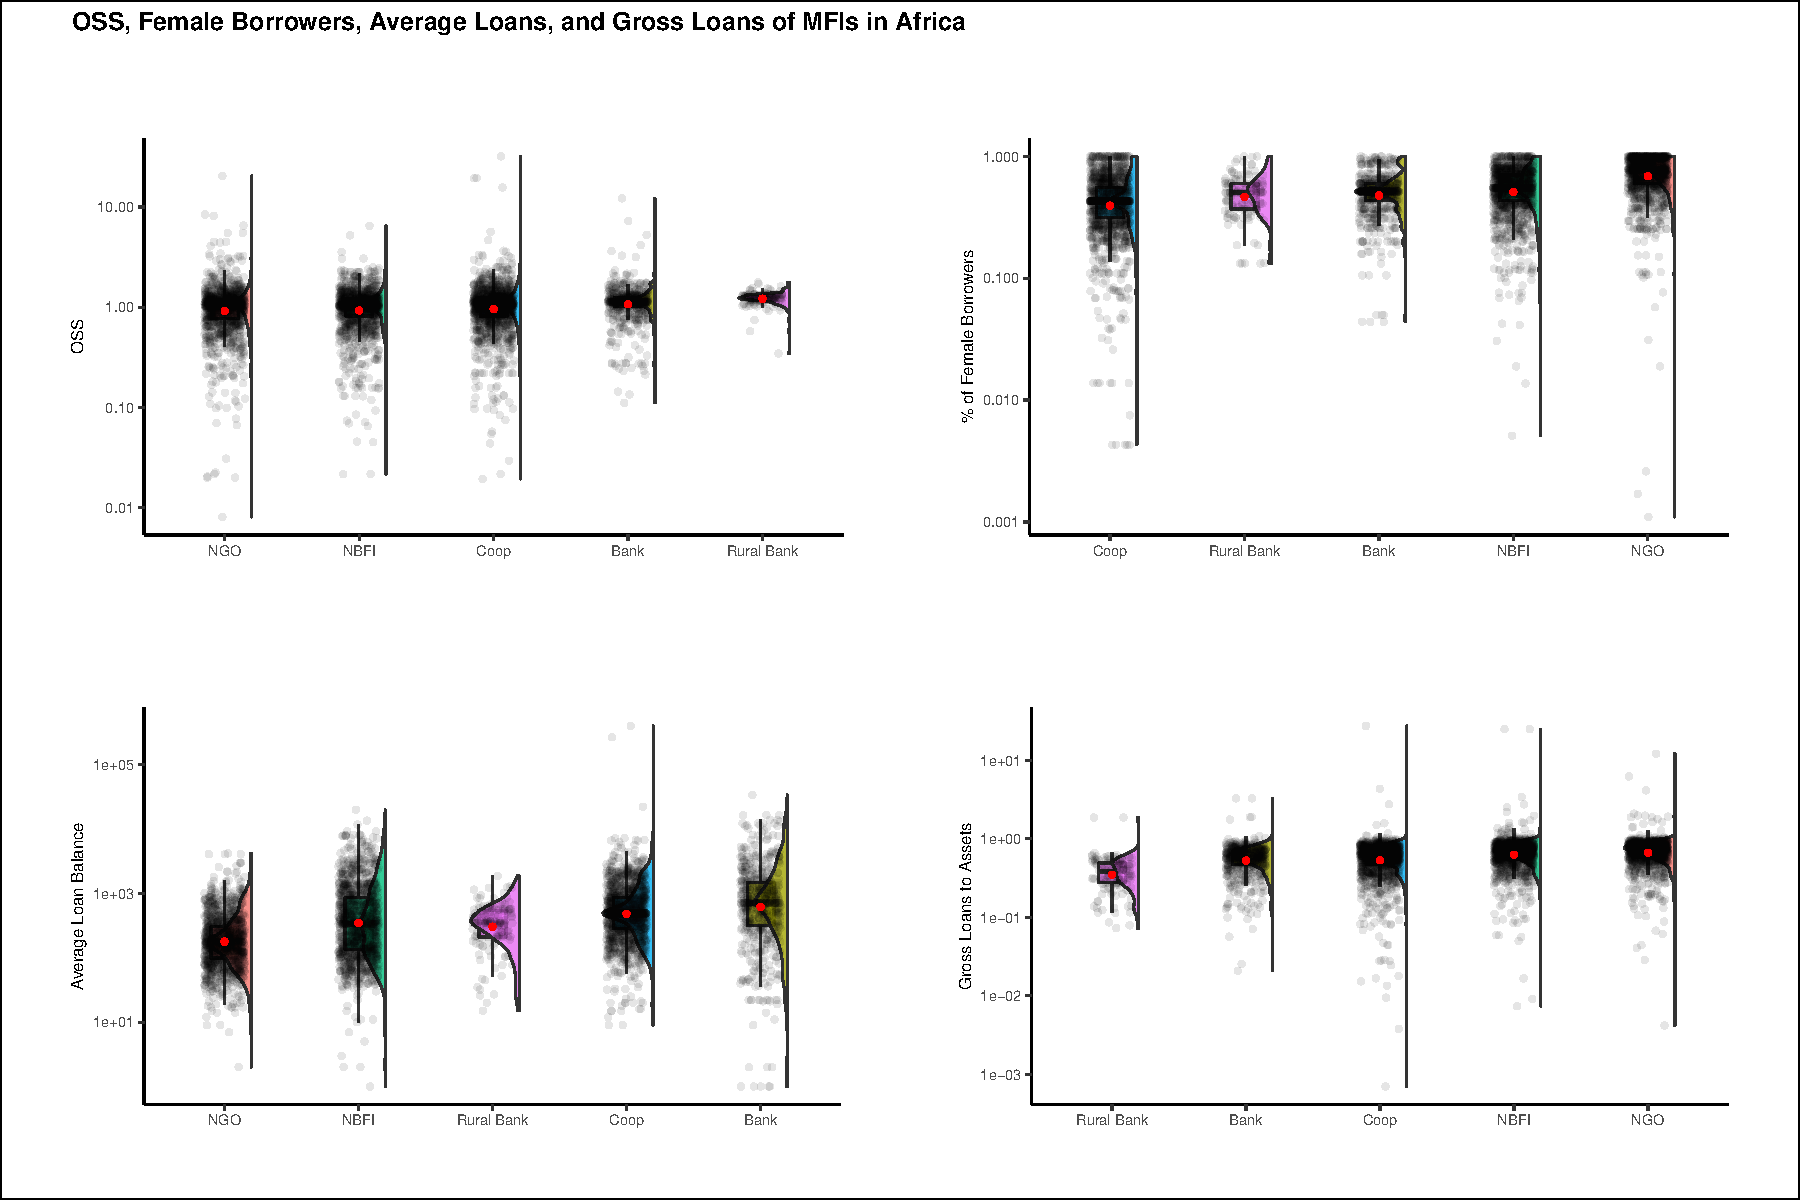
\includegraphics{finsoc_efficiency_files/figure-latex/unnamed-chunk-37-1.pdf}
\caption{Financial Sustainability and Social Performance Metrics for
MFIs in Africa}
\end{figure}

\end{landscape}

\begin{landscape}

\begin{table}[!htbp] \centering 
  \caption{Regression Output for Efficiency for Winsorized Data (Standard Errors in Brackets)} 
  \label{} 
\footnotesize 
\begin{tabular}{@{\extracolsep{5pt}}lD{.}{.}{-3} D{.}{.}{-3} D{.}{.}{-3} D{.}{.}{-3} D{.}{.}{-3} D{.}{.}{-3} } 
\\[-1.8ex]\hline 
\hline \\[-1.8ex] 
 & \multicolumn{6}{c}{\textit{Dependent variable:}} \\ 
\cline{2-7} 
\\[-1.8ex] & \multicolumn{6}{c}{depvar} \\ 
\\[-1.8ex] & \multicolumn{1}{c}{(1)} & \multicolumn{1}{c}{(2)} & \multicolumn{1}{c}{(3)} & \multicolumn{1}{c}{(4)} & \multicolumn{1}{c}{(5)} & \multicolumn{1}{c}{(6)}\\ 
\hline \\[-1.8ex] 
 currentlegalstatusBank &  &  &  & 0.125^{***} & -0.108^{***} & -0.077^{***} \\ 
  &  &  &  & (0.025) & (0.015) & (0.016) \\ 
  & & & & & & \\ 
 currentlegalstatusNBFI &  &  &  & 0.003 & -0.087^{***} & -0.082^{***} \\ 
  &  &  &  & (0.018) & (0.012) & (0.012) \\ 
  & & & & & & \\ 
 currentlegalstatusCoop & -0.0001 & 0.041 & 0.041 & 0.010 & -0.137^{***} & -0.126^{***} \\ 
  & (0.015) & (0.052) & (0.052) & (0.015) & (0.011) & (0.011) \\ 
  & & & & & & \\ 
 currentlegalstatusRural Bank &  &  &  & 0.066^{**} & -0.106^{***} & -0.080^{***} \\ 
  &  &  &  & (0.028) & (0.022) & (0.023) \\ 
  & & & & & & \\ 
 ageYoung & 0.003 & 0.002 & 0.002 & 0.001 & 0.001 & -0.001 \\ 
  & (0.002) & (0.005) & (0.005) & (0.003) & (0.005) & (0.005) \\ 
  & & & & & & \\ 
 ageMature & 0.005^{*} & -0.0002 & -0.0001 & 0.002 & -0.002 & -0.006 \\ 
  & (0.003) & (0.008) & (0.008) & (0.004) & (0.007) & (0.007) \\ 
  & & & & & & \\ 
 kkm & -0.002 & 0.001 & 0.001 & -0.00001 & -0.001 & -0.0002 \\ 
  & (0.001) & (0.003) & (0.003) & (0.001) & (0.002) & (0.002) \\ 
  & & & & & & \\ 
 asset\_structure & -0.078^{***} & 0.065 & 0.069 & -0.092^{***} & 0.034 & 0.024 \\ 
  & (0.020) & (0.044) & (0.045) & (0.025) & (0.041) & (0.043) \\ 
  & & & & & & \\ 
 pcrdbgdp & -0.003 & -0.020^{*} & -0.020^{*} & 0.0004 & -0.019^{***} & -0.016^{**} \\ 
  & (0.004) & (0.010) & (0.010) & (0.005) & (0.007) & (0.008) \\ 
  & & & & & & \\ 
 stmktcap & 0.005^{**} & -0.013^{***} & -0.011^{***} & 0.006^{**} & -0.0003 & 0.002 \\ 
  & (0.002) & (0.004) & (0.004) & (0.003) & (0.003) & (0.003) \\ 
  & & & & & & \\ 
 log(assets) & -0.162^{***} & 0.014 & 0.017 & -0.178^{***} & -0.034 & -0.046^{*} \\ 
  & (0.018) & (0.037) & (0.038) & (0.019) & (0.026) & (0.027) \\ 
  & & & & & & \\ 
\hline \\[-1.8ex] 
Model & Within & Within & Within & Random & Random & Random \\ 
Depvar & FinEff & SocEff & FinSocEff & FinEff & SocEff & FinSocEff \\ 
Data & Full & >=3 Years & >=5 Years & Full & >=3 Years & >=5 Years \\ 
Observations & \multicolumn{1}{c}{4,292} & \multicolumn{1}{c}{4,292} & \multicolumn{1}{c}{4,292} & \multicolumn{1}{c}{4,292} & \multicolumn{1}{c}{4,292} & \multicolumn{1}{c}{4,292} \\ 
R$^{2}$ & \multicolumn{1}{c}{0.062} & \multicolumn{1}{c}{0.043} & \multicolumn{1}{c}{0.041} & \multicolumn{1}{c}{0.132} & \multicolumn{1}{c}{0.632} & \multicolumn{1}{c}{0.627} \\ 
Adjusted R$^{2}$ & \multicolumn{1}{c}{-0.171} & \multicolumn{1}{c}{-0.196} & \multicolumn{1}{c}{-0.198} & \multicolumn{1}{c}{0.126} & \multicolumn{1}{c}{0.629} & \multicolumn{1}{c}{0.624} \\ 
F Statistic (df = 28; 3434) & \multicolumn{1}{c}{8.173$^{***}$} & \multicolumn{1}{c}{5.496$^{***}$} & \multicolumn{1}{c}{5.297$^{***}$} & \multicolumn{1}{c}{261.800$^{***}$} & \multicolumn{1}{c}{407.700$^{***}$} & \multicolumn{1}{c}{333.400$^{***}$} \\ 
\hline 
\hline \\[-1.8ex] 
\textit{Note:}  & \multicolumn{6}{r}{$^{*}$p$<$0.1; $^{**}$p$<$0.05; $^{***}$p$<$0.01} \\ 
\end{tabular} 
\end{table}

\end{landscape}

\end{document}
